% -*- mode: Noweb; noweb-code-mode: perl-mode -*-% ===> this file was generated automatically by noweave --- better not edit it
\documentclass[10pt]{article}
% 
% I'm trying to learn Literate Programming. I will use sgp2 as an LP exercise.
%
% The same document contains the code which will be generated with the proper filter:
%
%   pqtangle -L sgp2.tex
%
% The project documentation is also available from the same file:
%
%   latex sgp2.tex; dvips sgp2.dvi -o sgp2.ps  # to obtain the PS version 
%
%   pdflatex sgp2.tex;                         # to obtain the PS version
%
% $Id: sgp2.tex,v 1.9 2000-10-16 17:56:25 jabril Exp $
%  
\usepackage{noweb,multicol}
\usepackage[offset={0pt,0pt},hmargin={2.5cm,2cm},vmargin={1cm,0.25cm}]{geometry}
\usepackage{graphics}
\usepackage[dvips]{graphicx}
\noweboptions{smallcode}
% relax page breaking scheme
\def\nwendcode{\endtrivlist \endgroup}
\let\nwdocspar=\par

\newcommand{\sctn}[1]{\section{#1}}
\newcommand{\subsctn}[1]{\subsection{#1}}
\newcommand{\subsubsctn}[1]{\subsubsection{#1}}
\newcommand{\desc}[1]{\item[#1] \ \\}

\newcommand{\cd}[1]{\texttt{\textbf{#1}}} % program<code> font style definition
\newcommand{\cv}[1]{\texttt{\textsl{#1}}} % program<vars> font style definition
\newcommand{\cp}[1]{\textit{#1}} % program<vars> font style definition

\def\sgp{{\Tt{}sgp2}} % PROGRAM alias
\def\tbx{{\Tt{}tblastx}}
\def\bl{{\Tt{}blast}}
\def\gn{{\Tt{}genscan}}
\def\gi{{\Tt{}geneid}}
\def\sgpt{{\Tt{}sgp-2}}
\def\sgpo{{\Tt{}sgp-1}}
\def\scm{{\Tt{}scimog}}
\def\mit{{\Tt{}mit}}
\def\bi{{\Tt{}bi}}
 
% TITLE
\title{Sintenic Gene Prediction Tool}
\author{Roderic Guig\'o\\Josep F. Abril} %'

\begin{document}

\maketitle

\begin{center}
{\Large\sgp}\\[1ex]
{\large\verb+$Id: sgp2.tex,v 1.9 2000-10-16 17:56:25 jabril Exp $+}\\[2ex]
\end{center}

\begin{abstract}
The initial goal for Josep F. Abril will be to implement a \cd{perl} version of \sgp{}, which works like the current shell implementation. Secondary goals are to introduce myself into CVS (Concurrent Version Control) project management and Literate Programming (this document will serve as example).
\end{abstract}

\tableofcontents

\newpage

\sctn{Introduction}

\subsctn{On using comparative genomics to improve gene precition at genomic scale.}

Conservation in the genomic sequence of species at the appropiate
phylogenetic  distance may be indicative of conservation of sequence
function. We investigate here how sequence conservation may be
indicative of coding function, and develop program, SGP-2, which
integrates the results from \gi\ and \tbx\ to produce gene predictions
when comparing human/mouse sintenynic regions.
We set up a number benchmark data sets,
in which we test SGP-2 against ``ab initio'' programs, sequence
similarity based programs, and other hibrid programs. 

\subsctn{Data Sets}
So far, we used three different human/mouse data sets.
\begin{description}
\item[scimog] 39 pairs of single gene homologous sequences. Obtained by
merging the set by \cite{jarborg:1999a} and the set obtained by us at IMIM.
\item[mit] 110 pairs of single gene homologous sequences. Obtained
from the 117 pairs in \cite{batzoglou:2000a}
\item[bi] 3 pairs of genomic pairs encoding multiple genes. Obtained
by Webb Miller/Thomas Wiehe.
\end{description}

\subsctn{Programs}
\begin{description}
\item[genscan] default parameters
\item[geneid] new released version. default parameters
\item[tblastx] WU (see summer 1999 report)
\item[rosseta] {\tt www.theory.lcs.mit.edu/crossspecies}
\end{description}
 
\subsctn{SGP-2}
Figure \ref{fig:algo2} describes the approach in algo2.  Given two
genomic sequences

\begin{enumerate}
\item mask the sequences using RepeatMasker.
\item run \tbx\ of one sequence agains the other. We run \tbx\
with the option {\tt nogap}, and using blosum62 and with score for
aligning to stop codon set to -500
\item ``project'' the similarity regions onto each sequence
\item  run \gi\ on each sequence with the projected similarity regions
given with the {\tt -S} option
\end{enumerate}

A prototype of {\sgp} already exists.

\begin{figure}
\begin{center}
\framebox{
\includegraphics[width=0.85\linewidth, trim= 10 10 20 10, clip]{../docs/figs/algo2.ps}
}
\end{center}
\caption{ }
\label{fig:algo2}
\end{figure}

\subsctn{Results}

\subsubsctn{scimog}

\input ../docs/tables/Table-scimog.tex


\subsubsctn{mit}

\input ../docs/tables/Table-mit.tex

\subsubsctn{bi}
Only one sequence from each pair is used to report accuracy, because
doubts on the annnotation of the other in the pair

\input ../docs/tables/Table-bi.tex
 
\newpage

\sctn{Perl Implementation}

\subsctn{Program Basic Outline}

Our initial program outline (our root chunk) looks like:\\[1ex]

\nwfilename{./sgp2.nw}\nwbegincode{1}\sublabel{NWsgp9-sgp7-1}\nwmargintag{{\nwtagstyle{}\subpageref{NWsgp9-sgp7-1}}}\moddef{sgp2.pl~{\nwtagstyle{}\subpageref{NWsgp9-sgp7-1}}}\endmoddef\nwstartdeflinemarkup\nwenddeflinemarkup
\LA{}shebang~{\nwtagstyle{}\subpageref{NWsgp9-she7-1}}\RA{}
\LA{}version control~{\nwtagstyle{}\subpageref{NWsgp9-verF-1}}\RA{}
\LA{}declare uses~{\nwtagstyle{}\subpageref{NWsgp9-decC-1}}\RA{}

### VARS ###

\LA{}define defaults~{\nwtagstyle{}\subpageref{NWsgp9-defF-1}}\RA{}
\LA{}declare variables~{\nwtagstyle{}\subpageref{NWsgp9-decH-1}}\RA{}

### SUBS ###

\LA{}global subroutines~{\nwtagstyle{}\subpageref{NWsgp9-gloI-1}}\RA{}
\LA{}get options~{\nwtagstyle{}\subpageref{NWsgp9-getB-1}}\RA{}

### MAIN SUBS ###

\LA{}run blast~{\nwtagstyle{}\subpageref{NWsgp9-run9-1}}\RA{}
\LA{}extract HSPs~{\nwtagstyle{}\subpageref{NWsgp9-extC-1}}\RA{}
\LA{}run geneid~{\nwtagstyle{}\subpageref{NWsgp9-runA-1}}\RA{}
\LA{}graphical output~{\nwtagstyle{}\subpageref{NWsgp9-graG-1}}\RA{}

### MAIN LOOP ###

\LA{}Main Loop~{\nwtagstyle{}\subpageref{NWsgp9-Mai9-1}}\RA{}

### EOF ###

\LA{}POD man page trailer~{\nwtagstyle{}\subpageref{NWsgp9-PODK-1}}\RA{}
\nwnotused{sgp2.pl}\nwendcode{}\nwbegindocs{2}% 

{\Tt{}\LA{}declare uses~{\nwtagstyle{}\subpageref{NWsgp9-decC-1}}\RA{}} will cover all the modules (standard or not) that our program will need in the coresponding section.
{\Tt{}\LA{}declare variables~{\nwtagstyle{}\subpageref{NWsgp9-decH-1}}\RA{}} collect all the variables that need to be declared global within this program.

\nwenddocs{}\nwbegincode{3}\sublabel{NWsgp9-she7-1}\nwmargintag{{\nwtagstyle{}\subpageref{NWsgp9-she7-1}}}\moddef{shebang~{\nwtagstyle{}\subpageref{NWsgp9-she7-1}}}\endmoddef\nwstartdeflinemarkup\nwusesondefline{\\{NWsgp9-sgp7-1}}\nwenddeflinemarkup
#!/usr/bin/perl -w
\LA{}copyleft~{\nwtagstyle{}\subpageref{NWsgp9-cop8-1}}\RA{}
my $Start = time;
\nwused{\\{NWsgp9-sgp7-1}}\nwendcode{}\nwbegindocs{4} %def $Start

'\cd{perl -w}' prints all sorts of useful and interesting warning messages at compile time.

{\Tt{}{\$}Start} %$
contains program starting time (seconds since \textsc{Unix} ``epoch''), which will be used by timing function to calculate for how long was running our program.

\nwenddocs{}\nwbegincode{5}\sublabel{NWsgp9-verF-1}\nwmargintag{{\nwtagstyle{}\subpageref{NWsgp9-verF-1}}}\moddef{version control~{\nwtagstyle{}\subpageref{NWsgp9-verF-1}}}\endmoddef\nwstartdeflinemarkup\nwusesondefline{\\{NWsgp9-sgp7-1}}\nwenddeflinemarkup
my $PROGRAM = "sgp2";
my @tmp_ver = split / +/, ' $Id: sgp2.tex,v 1.9 2000-10-16 17:56:25 jabril Exp $ ';
my $VERSION = "v$tmp_ver[3] [$tmp_ver[4] $tmp_ver[5] $tmp_ver[7]]";
\nwindexdefn{\nwixident{{\$}PROGRAM}}{:doPROGRAM}{NWsgp9-verF-1}\nwindexdefn{\nwixident{{\$}VERSION}}{:doVERSION}{NWsgp9-verF-1}\nwindexdefn{\nwixident{@tmp{\_}ver}}{@tmp:unver}{NWsgp9-verF-1}\eatline
\nwused{\\{NWsgp9-sgp7-1}}\nwidentdefs{\\{{\nwixident{{\$}PROGRAM}}{:doPROGRAM}}\\{{\nwixident{@tmp{\_}ver}}{@tmp:unver}}\\{{\nwixident{{\$}VERSION}}{:doVERSION}}}\nwendcode{}\nwbegindocs{6}\nwdocspar
Take into account that here is shown {\Tt{}sgp2.nw} versions, but once the perl script is extracted ({\Tt{}noweb}) and commited (CVS) then it follows {\Tt{}sgp2.pl} version numbering.

\nwenddocs{}\nwbegincode{7}\sublabel{NWsgp9-decC-1}\nwmargintag{{\nwtagstyle{}\subpageref{NWsgp9-decC-1}}}\moddef{declare uses~{\nwtagstyle{}\subpageref{NWsgp9-decC-1}}}\endmoddef\nwstartdeflinemarkup\nwusesondefline{\\{NWsgp9-sgp7-1}}\nwprevnextdefs{\relax}{NWsgp9-decC-2}\nwenddeflinemarkup
use strict;
\nwalsodefined{\\{NWsgp9-decC-2}\\{NWsgp9-decC-3}\\{NWsgp9-decC-4}\\{NWsgp9-decC-5}}\nwused{\\{NWsgp9-sgp7-1}}\nwendcode{}\nwbegindocs{8}\nwdocspar

``\cd{use strict;}'' restricts unsafe constructs, like attempting to use missed symbolic references ('\cv{refs}'), undeclared variables ('\cv{vars}') or not predeclared subroutine ('\cv{subs}').

\subsctn{Main Program Loop}

\nwenddocs{}\nwbegincode{9}\sublabel{NWsgp9-Mai9-1}\nwmargintag{{\nwtagstyle{}\subpageref{NWsgp9-Mai9-1}}}\moddef{Main Loop~{\nwtagstyle{}\subpageref{NWsgp9-Mai9-1}}}\endmoddef\nwstartdeflinemarkup\nwusesondefline{\\{NWsgp9-sgp7-1}}\nwenddeflinemarkup
# get options
&Which_Options();
# main external program calls
DOBLAST: do \{
    &Run_Blast() if $blast_flg;
    &Extract_HSP();
\} if $hsps_flg;
&Run_geneid()  if $geneid_flg;
&Make_Plots()  if $plots_flg; 
# removing temporary files
&clean_tmp();
# timing and exit
&get_exec_time(time);
exit(0);
\nwused{\\{NWsgp9-sgp7-1}}\nwidentuses{\\{{\nwixident{{\$}blast{\_}flg}}{:doblast:unflg}}\\{{\nwixident{{\&}clean{\_}tmp}}{:amclean:untmp}}\\{{\nwixident{{\&}Extract{\_}HSP}}{:amExtract:unHSP}}\\{{\nwixident{{\$}geneid{\_}flg}}{:dogeneid:unflg}}\\{{\nwixident{{\&}get{\_}exec{\_}time}}{:amget:unexec:untime}}\\{{\nwixident{{\$}hsps{\_}flg}}{:dohsps:unflg}}\\{{\nwixident{{\&}Make{\_}Plots}}{:amMake:unPlots}}\\{{\nwixident{{\$}plots{\_}flg}}{:doplots:unflg}}\\{{\nwixident{{\&}Run{\_}Blast}}{:amRun:unBlast}}\\{{\nwixident{{\&}Run{\_}geneid}}{:amRun:ungeneid}}\\{{\nwixident{{\&}Which{\_}Options}}{:amWhich:unOptions}}}\nwindexuse{\nwixident{{\$}blast{\_}flg}}{:doblast:unflg}{NWsgp9-Mai9-1}\nwindexuse{\nwixident{{\&}clean{\_}tmp}}{:amclean:untmp}{NWsgp9-Mai9-1}\nwindexuse{\nwixident{{\&}Extract{\_}HSP}}{:amExtract:unHSP}{NWsgp9-Mai9-1}\nwindexuse{\nwixident{{\$}geneid{\_}flg}}{:dogeneid:unflg}{NWsgp9-Mai9-1}\nwindexuse{\nwixident{{\&}get{\_}exec{\_}time}}{:amget:unexec:untime}{NWsgp9-Mai9-1}\nwindexuse{\nwixident{{\$}hsps{\_}flg}}{:dohsps:unflg}{NWsgp9-Mai9-1}\nwindexuse{\nwixident{{\&}Make{\_}Plots}}{:amMake:unPlots}{NWsgp9-Mai9-1}\nwindexuse{\nwixident{{\$}plots{\_}flg}}{:doplots:unflg}{NWsgp9-Mai9-1}\nwindexuse{\nwixident{{\&}Run{\_}Blast}}{:amRun:unBlast}{NWsgp9-Mai9-1}\nwindexuse{\nwixident{{\&}Run{\_}geneid}}{:amRun:ungeneid}{NWsgp9-Mai9-1}\nwindexuse{\nwixident{{\&}Which{\_}Options}}{:amWhich:unOptions}{NWsgp9-Mai9-1}\nwendcode{}\nwbegindocs{10}\nwdocspar

\subsubsctn{Default values setting}

\nwenddocs{}\nwbegincode{11}\sublabel{NWsgp9-defF-1}\nwmargintag{{\nwtagstyle{}\subpageref{NWsgp9-defF-1}}}\moddef{define defaults~{\nwtagstyle{}\subpageref{NWsgp9-defF-1}}}\endmoddef\nwstartdeflinemarkup\nwusesondefline{\\{NWsgp9-sgp7-1}}\nwprevnextdefs{\relax}{NWsgp9-defF-2}\nwenddeflinemarkup
# some defaults
my $S_CUTOFF = 50;
my $SCF = 12; # substract to tblastx scores S_CUTOFF - SCF;
\nwindexdefn{\nwixident{{\$}S{\_}CUTOFF}}{:doS:unCUTOFF}{NWsgp9-defF-1}\nwindexdefn{\nwixident{{\$}SCF}}{:doSCF}{NWsgp9-defF-1}\eatline
\nwalsodefined{\\{NWsgp9-defF-2}}\nwused{\\{NWsgp9-sgp7-1}}\nwidentdefs{\\{{\nwixident{{\$}SCF}}{:doSCF}}\\{{\nwixident{{\$}S{\_}CUTOFF}}{:doS:unCUTOFF}}}\nwendcode{}\nwbegindocs{12}\nwdocspar
{\Tt{}{\$}S{\_}CUTOFF} and {\Tt{}{\$}SCF} are used when the program parses {\Tt{}tblastx} output to rescore HSPs by subtracting {\Tt{}{\$}S{\_}CUTOFF} - {\Tt{}{\$}SCF} to HSP scores.

\nwenddocs{}\nwbegincode{13}\sublabel{NWsgp9-defF-2}\nwmargintag{{\nwtagstyle{}\subpageref{NWsgp9-defF-2}}}\moddef{define defaults~{\nwtagstyle{}\subpageref{NWsgp9-defF-1}}}\plusendmoddef\nwstartdeflinemarkup\nwusesondefline{\\{NWsgp9-sgp7-1}}\nwprevnextdefs{NWsgp9-defF-1}{\relax}\nwenddeflinemarkup
# setting paths
my $SGP2   = $ENV\{'SGP'\};
my $SGP2bin = "$SGP2/bin";
my $SGP2param = "$SGP2bin/param";
my $TMP    = '/tmp';
my $TMPROOT = "sgp2_$$";
my $SGPTMP = "$TMP/$TMPROOT";
\LA{}trap temporary files~{\nwtagstyle{}\subpageref{NWsgp9-traK-1}}\RA{}
\nwindexdefn{\nwixident{{\$}SGP2}}{:doSGP2}{NWsgp9-defF-2}\nwindexdefn{\nwixident{{\$}SGP2bin}}{:doSGP2bin}{NWsgp9-defF-2}\nwindexdefn{\nwixident{{\$}SGP2param}}{:doSGP2param}{NWsgp9-defF-2}\nwindexdefn{\nwixident{{\$}TMP}}{:doTMP}{NWsgp9-defF-2}\nwindexdefn{\nwixident{{\$}TMPROOT}}{:doTMPROOT}{NWsgp9-defF-2}\nwindexdefn{\nwixident{{\$}SGPTMP}}{:doSGPTMP}{NWsgp9-defF-2}\eatline
\nwused{\\{NWsgp9-sgp7-1}}\nwidentdefs{\\{{\nwixident{{\$}SGP2}}{:doSGP2}}\\{{\nwixident{{\$}SGP2bin}}{:doSGP2bin}}\\{{\nwixident{{\$}SGP2param}}{:doSGP2param}}\\{{\nwixident{{\$}SGPTMP}}{:doSGPTMP}}\\{{\nwixident{{\$}TMP}}{:doTMP}}\\{{\nwixident{{\$}TMPROOT}}{:doTMPROOT}}}\nwendcode{}\nwbegindocs{14}%$

{\Tt{}{\$}SGP2} %$
defines main path to {\sgp} binaries, scripts and params.
{\Tt{}{\$}TMP} %$ 
is the temporary working directory, and {\Tt{}{\$}SGPTMP} %$ 
contains the prefix for temporal files that is set different by adding the process ID ({\Tt{}{\$}{\$}} in plain {\Tt{}perl}, if ``{\Tt{}use\ English;}'' is given it can also be defined as {\Tt{}{\$}PROCESS{\_}ID} or {\Tt{}{\$}PID}).

\nwenddocs{}\nwbegincode{15}\sublabel{NWsgp9-traK-1}\nwmargintag{{\nwtagstyle{}\subpageref{NWsgp9-traK-1}}}\moddef{trap temporary files~{\nwtagstyle{}\subpageref{NWsgp9-traK-1}}}\endmoddef\nwstartdeflinemarkup\nwusesondefline{\\{NWsgp9-defF-2}}\nwenddeflinemarkup
$SIG\{INT\}  = \\&trap_signals;
$SIG\{QUIT\} = \\&trap_signals;
$SIG\{TERM\} = \\&trap_signals;
$SIG\{CHLD\} = 'IGNORE';
sub trap_signals() \{
    # opendir(TDIR, $TMP) or &go_to_die("Can't open directory $TMP: $!");
    # while (defined(my $file = readdir(TDIR)))
    &clean_tmp();
    &go_to_die("WARNING !!! $PROGRAM has been stopped by user.");
\}
\nwused{\\{NWsgp9-defF-2}}\nwidentuses{\\{{\nwixident{{\&}clean{\_}tmp}}{:amclean:untmp}}\\{{\nwixident{{\&}go{\_}to{\_}die}}{:amgo:unto:undie}}\\{{\nwixident{{\$}PROGRAM}}{:doPROGRAM}}\\{{\nwixident{{\$}TMP}}{:doTMP}}}\nwindexuse{\nwixident{{\&}clean{\_}tmp}}{:amclean:untmp}{NWsgp9-traK-1}\nwindexuse{\nwixident{{\&}go{\_}to{\_}die}}{:amgo:unto:undie}{NWsgp9-traK-1}\nwindexuse{\nwixident{{\$}PROGRAM}}{:doPROGRAM}{NWsgp9-traK-1}\nwindexuse{\nwixident{{\$}TMP}}{:doTMP}{NWsgp9-traK-1}\nwendcode{}\nwbegindocs{16}%$

The following signals are trapped by our signal handler routine:
\begin{itemize}
\item {\Tt{}SIGINT} is normally triggered by Ctrl-C, requesting that a process interrupt what it's doing.%'
\item {\Tt{}SIGQUIT} is also generated by a terminal, usually Ctrl-$\backslash$, generating a core dump.
\item {\Tt{}SIGTERM} is sent by {\Tt{}kill} shell command when no signal name is explicitly given (think of it as a polite request for a process to die). 
\end{itemize}

\subsubsctn{Parsing Command-line Options}

\nwenddocs{}\nwbegincode{17}\sublabel{NWsgp9-decC-2}\nwmargintag{{\nwtagstyle{}\subpageref{NWsgp9-decC-2}}}\moddef{declare uses~{\nwtagstyle{}\subpageref{NWsgp9-decC-1}}}\plusendmoddef\nwstartdeflinemarkup\nwusesondefline{\\{NWsgp9-sgp7-1}}\nwprevnextdefs{NWsgp9-decC-1}{NWsgp9-decC-3}\nwenddeflinemarkup
use Getopt::Long;
Getopt::Long::Configure qw/ bundling pass_through /;
\nwused{\\{NWsgp9-sgp7-1}}\nwendcode{}\nwbegindocs{18}\nwdocspar

\begin{description}
\desc{\cd{use Getopt::Long;}} This module implements an extended getopt function called \cd{GetOptions()}. This function adheres to the POSIX syntax for command line options, with GNU extensions. In general, this means that options having long names instead of single letters are introduced with a double dash "-\/-". 

\desc{\cd{Getopt::Long::Configure qw(} \cv{bundling} \cv{pass\_through} \cd{);}} \cd{GetOptions} can be configured by calling subroutine \cd{Getopt::Long::Configure}. This subroutine takes a list of quoted strings, each specifying a configuration option to be set. Options can be reset by prefixing with '\cv{no\_}'. 

 \begin{description}
 \desc{\cv{bundling}} Support for bundling of command line options, as was the case with the more traditional single-letter approach (introduced with a single dash "-"), is provided but not enabled by default. 

 \desc{\cv{pass\_through}} Unknown options are passed through in \cd{@ARGV} instead of being flagged as errors. This makes it possible to write wrapper scripts that process only part of the user supplied options, and passes the remaining options to some other program.
 \end{description}
\end{description}

\nwenddocs{}\nwbegincode{19}\sublabel{NWsgp9-decH-1}\nwmargintag{{\nwtagstyle{}\subpageref{NWsgp9-decH-1}}}\moddef{declare variables~{\nwtagstyle{}\subpageref{NWsgp9-decH-1}}}\endmoddef\nwstartdeflinemarkup\nwusesondefline{\\{NWsgp9-sgp7-1}}\nwprevnextdefs{\relax}{NWsgp9-decH-2}\nwenddeflinemarkup
# GetOptions Variables
my ( $Seq1, $Seq2, $geneid_opt, $geneid_param, 
     $blast_opt, $score_cutoff, $shrink, $tbx,
     $hsp, $ofn, $ps_output, $savefiles_flg, $verbose_flg, $help_flg
     ) = ( undef, undef, undef, undef, undef, undef,
           undef, undef, undef, undef, undef, 0, 0, 0 );
\nwindexdefn{\nwixident{{\$}Seq1}}{:doSeq1}{NWsgp9-decH-1}\nwindexdefn{\nwixident{{\$}Seq2}}{:doSeq2}{NWsgp9-decH-1}\nwindexdefn{\nwixident{{\$}geneid{\_}opt}}{:dogeneid:unopt}{NWsgp9-decH-1}\nwindexdefn{\nwixident{{\$}geneid{\_}param}}{:dogeneid:unparam}{NWsgp9-decH-1}\nwindexdefn{\nwixident{{\$}blast{\_}opt}}{:doblast:unopt}{NWsgp9-decH-1}\nwindexdefn{\nwixident{{\$}score{\_}cutoff}}{:doscore:uncutoff}{NWsgp9-decH-1}\nwindexdefn{\nwixident{{\$}shrink}}{:doshrink}{NWsgp9-decH-1}\nwindexdefn{\nwixident{{\$}tbx}}{:dotbx}{NWsgp9-decH-1}\nwindexdefn{\nwixident{{\$}hsp}}{:dohsp}{NWsgp9-decH-1}\nwindexdefn{\nwixident{{\$}ofn}}{:doofn}{NWsgp9-decH-1}\nwindexdefn{\nwixident{{\$}ps{\_}output}}{:dops:unoutput}{NWsgp9-decH-1}\nwindexdefn{\nwixident{{\$}savefiles{\_}flg}}{:dosavefiles:unflg}{NWsgp9-decH-1}\nwindexdefn{\nwixident{{\$}verbose{\_}flg}}{:doverbose:unflg}{NWsgp9-decH-1}\nwindexdefn{\nwixident{{\$}help{\_}flg}}{:dohelp:unflg}{NWsgp9-decH-1}\eatline
\nwalsodefined{\\{NWsgp9-decH-2}\\{NWsgp9-decH-3}\\{NWsgp9-decH-4}\\{NWsgp9-decH-5}\\{NWsgp9-decH-6}\\{NWsgp9-decH-7}}\nwused{\\{NWsgp9-sgp7-1}}\nwidentdefs{\\{{\nwixident{{\$}blast{\_}opt}}{:doblast:unopt}}\\{{\nwixident{{\$}geneid{\_}opt}}{:dogeneid:unopt}}\\{{\nwixident{{\$}geneid{\_}param}}{:dogeneid:unparam}}\\{{\nwixident{{\$}help{\_}flg}}{:dohelp:unflg}}\\{{\nwixident{{\$}hsp}}{:dohsp}}\\{{\nwixident{{\$}ofn}}{:doofn}}\\{{\nwixident{{\$}ps{\_}output}}{:dops:unoutput}}\\{{\nwixident{{\$}savefiles{\_}flg}}{:dosavefiles:unflg}}\\{{\nwixident{{\$}score{\_}cutoff}}{:doscore:uncutoff}}\\{{\nwixident{{\$}Seq1}}{:doSeq1}}\\{{\nwixident{{\$}Seq2}}{:doSeq2}}\\{{\nwixident{{\$}shrink}}{:doshrink}}\\{{\nwixident{{\$}tbx}}{:dotbx}}\\{{\nwixident{{\$}verbose{\_}flg}}{:doverbose:unflg}}}\nwendcode{}\nwbegindocs{20}\nwdocspar
Those variables will receive the values passed from command-line options in {\Tt{}Which{\_}Options()} function. We set them as {\Tt{}undef} to check after {\Tt{}Which{\_}Options()} if they have received any value (with {\Tt{}defined()} function).

\nwenddocs{}\nwbegincode{21}\sublabel{NWsgp9-getB-1}\nwmargintag{{\nwtagstyle{}\subpageref{NWsgp9-getB-1}}}\moddef{get options~{\nwtagstyle{}\subpageref{NWsgp9-getB-1}}}\endmoddef\nwstartdeflinemarkup\nwusesondefline{\\{NWsgp9-sgp7-1}}\nwenddeflinemarkup
# Parsing command-line options and processing its parameters.
\LA{}getopts subs~{\nwtagstyle{}\subpageref{NWsgp9-getC-1}}\RA{}
sub Which_Options() \{
    GetOptions( 
                "1=s"      => \\$Seq1         , # seqfile_1
                "2=s"      => \\$Seq2         , # seqfile_2
                "g=s"      => \\$geneid_opt   , # geneid options      
                "P=s"      => \\$geneid_param , # geneid parameter file 
                "o=s"      => \\$blast_opt    , # tblastx options 
                "c=f"      => \\$score_cutoff , # tblastx score cutoff 
                "s=f"      => \\$shrink       , # shrink hsp's by
                "t=s"      => \\$tbx          , # read tblastx from file
                "f=s"      => \\$hsp          , # read HSP files in directory
                "k=s"      => \\$ofn          , # intermediate filename
                "p=s"      => \\$ps_output    , # postscript output 
                "v"        => \\$verbose_flg  , # verbose    
                "h|help|?" => \\$help_flg     , # print help
                );
    &prt_Help if $help_flg;
    &prt_Header("Processsing Command-Line Options") if $verbose_flg;
    \LA{}set flags-vars~{\nwtagstyle{}\subpageref{NWsgp9-setE-1}}\RA{}
\} # sub Which_Options
\nwindexdefn{\nwixident{{\&}Which{\_}Options}}{:amWhich:unOptions}{NWsgp9-getB-1}\eatline
\nwused{\\{NWsgp9-sgp7-1}}\nwidentdefs{\\{{\nwixident{{\&}Which{\_}Options}}{:amWhich:unOptions}}}\nwidentuses{\\{{\nwixident{{\$}blast{\_}opt}}{:doblast:unopt}}\\{{\nwixident{{\$}geneid{\_}opt}}{:dogeneid:unopt}}\\{{\nwixident{{\$}geneid{\_}param}}{:dogeneid:unparam}}\\{{\nwixident{{\$}help{\_}flg}}{:dohelp:unflg}}\\{{\nwixident{{\$}hsp}}{:dohsp}}\\{{\nwixident{{\$}ofn}}{:doofn}}\\{{\nwixident{{\&}prt{\_}Help}}{:amprt:unHelp}}\\{{\nwixident{{\$}ps{\_}output}}{:dops:unoutput}}\\{{\nwixident{{\$}score{\_}cutoff}}{:doscore:uncutoff}}\\{{\nwixident{{\$}Seq1}}{:doSeq1}}\\{{\nwixident{{\$}Seq2}}{:doSeq2}}\\{{\nwixident{{\$}shrink}}{:doshrink}}\\{{\nwixident{{\$}tbx}}{:dotbx}}\\{{\nwixident{{\$}verbose{\_}flg}}{:doverbose:unflg}}}\nwindexuse{\nwixident{{\$}blast{\_}opt}}{:doblast:unopt}{NWsgp9-getB-1}\nwindexuse{\nwixident{{\$}geneid{\_}opt}}{:dogeneid:unopt}{NWsgp9-getB-1}\nwindexuse{\nwixident{{\$}geneid{\_}param}}{:dogeneid:unparam}{NWsgp9-getB-1}\nwindexuse{\nwixident{{\$}help{\_}flg}}{:dohelp:unflg}{NWsgp9-getB-1}\nwindexuse{\nwixident{{\$}hsp}}{:dohsp}{NWsgp9-getB-1}\nwindexuse{\nwixident{{\$}ofn}}{:doofn}{NWsgp9-getB-1}\nwindexuse{\nwixident{{\&}prt{\_}Help}}{:amprt:unHelp}{NWsgp9-getB-1}\nwindexuse{\nwixident{{\$}ps{\_}output}}{:dops:unoutput}{NWsgp9-getB-1}\nwindexuse{\nwixident{{\$}score{\_}cutoff}}{:doscore:uncutoff}{NWsgp9-getB-1}\nwindexuse{\nwixident{{\$}Seq1}}{:doSeq1}{NWsgp9-getB-1}\nwindexuse{\nwixident{{\$}Seq2}}{:doSeq2}{NWsgp9-getB-1}\nwindexuse{\nwixident{{\$}shrink}}{:doshrink}{NWsgp9-getB-1}\nwindexuse{\nwixident{{\$}tbx}}{:dotbx}{NWsgp9-getB-1}\nwindexuse{\nwixident{{\$}verbose{\_}flg}}{:doverbose:unflg}{NWsgp9-getB-1}\nwendcode{}\nwbegindocs{22}%$

In {\Tt{}GetOptions()} function, sufixing an option with '=s' implies that it will require a mandatory string parameter, with '=f' the option must be provided with a real number. The following variables need a filename: {\Tt{}{\$}geneid{\_}param} {\Tt{}{\$}tbx} {\Tt{}{\$}hsp} {\Tt{}{\$}ofn} {\Tt{}{\$}ps{\_}output}.
 
\nwenddocs{}\nwbegincode{23}\sublabel{NWsgp9-getC-1}\nwmargintag{{\nwtagstyle{}\subpageref{NWsgp9-getC-1}}}\moddef{getopts subs~{\nwtagstyle{}\subpageref{NWsgp9-getC-1}}}\endmoddef\nwstartdeflinemarkup\nwusesondefline{\\{NWsgp9-getB-1}}\nwenddeflinemarkup
# Checking input sequence files
sub exists_file() \{
    my @files = @_;
    my ($n, $r) = ('', 0);
    foreach $n (@files) \{
        $r++ if (-e $n);
    \};
    return $r;
\}
sub check_fasta_format() \{
    my $file = $_[0];
    my ($n, $c) = (undef, 0);
    open(TMP,"< $file");
    while (<TMP>) \{
                next unless /^>/;
        />(\\S+)\\b/ && do \{
            $n = $1;
            $c++;
            next unless $c>1;
        \};
                &go_to_die("FATAL ERROR !!! Multiple locus names found.\\n  File '$file' must contain only one sequence definition.\\n");
    \}
    &go_to_die("FATAL ERROR !!! There is no '>' line, locus name not found.\\n  Please, verify your fasta file '$file'\\n") unless defined($n);
    return $n;
\}
\nwindexdefn{\nwixident{{\&}exists{\_}file}}{:amexists:unfile}{NWsgp9-getC-1}\nwindexdefn{\nwixident{{\&}check{\_}fasta{\_}format}}{:amcheck:unfasta:unformat}{NWsgp9-getC-1}\eatline
\nwused{\\{NWsgp9-getB-1}}\nwidentdefs{\\{{\nwixident{{\&}check{\_}fasta{\_}format}}{:amcheck:unfasta:unformat}}\\{{\nwixident{{\&}exists{\_}file}}{:amexists:unfile}}}\nwidentuses{\\{{\nwixident{{\&}go{\_}to{\_}die}}{:amgo:unto:undie}}}\nwindexuse{\nwixident{{\&}go{\_}to{\_}die}}{:amgo:unto:undie}{NWsgp9-getC-1}\nwendcode{}\nwbegindocs{24}%$

{\Tt{}exists{\_}file()} : Given a list of filenames, this function returns how many among them does exist.
{\Tt{}check{\_}fasta{\_}format()} : For a given file, returns the \textit{locus} name if file is in {\Tt{}fasta} format, else program dies.

\nwenddocs{}\nwbegincode{25}\sublabel{NWsgp9-decC-3}\nwmargintag{{\nwtagstyle{}\subpageref{NWsgp9-decC-3}}}\moddef{declare uses~{\nwtagstyle{}\subpageref{NWsgp9-decC-1}}}\plusendmoddef\nwstartdeflinemarkup\nwusesondefline{\\{NWsgp9-sgp7-1}}\nwprevnextdefs{NWsgp9-decC-2}{NWsgp9-decC-4}\nwenddeflinemarkup
use File::Basename;
\nwused{\\{NWsgp9-sgp7-1}}\nwendcode{}\nwbegindocs{26}\nwdocspar

This standard module contains routines to split up a filename. {\Tt{}basename} is provided for programmer compatibility with the same name \textsc{Unix} shell command.

\nwenddocs{}\nwbegincode{27}\sublabel{NWsgp9-decH-2}\nwmargintag{{\nwtagstyle{}\subpageref{NWsgp9-decH-2}}}\moddef{declare variables~{\nwtagstyle{}\subpageref{NWsgp9-decH-1}}}\plusendmoddef\nwstartdeflinemarkup\nwusesondefline{\\{NWsgp9-sgp7-1}}\nwprevnextdefs{NWsgp9-decH-1}{NWsgp9-decH-3}\nwenddeflinemarkup
# sequence files
my ($Seq1_Name, $Seq2_Name, $Loc1, $Loc2, $SGPtmp1, $SGPtmp2, $SGPtmpG);
\nwindexdefn{\nwixident{{\$}Seq1{\_}Name}}{:doSeq1:unName}{NWsgp9-decH-2}\nwindexdefn{\nwixident{{\$}Seq2{\_}Name}}{:doSeq2:unName}{NWsgp9-decH-2}\nwindexdefn{\nwixident{{\$}Loc1}}{:doLoc1}{NWsgp9-decH-2}\nwindexdefn{\nwixident{{\$}Loc2}}{:doLoc2}{NWsgp9-decH-2}\nwindexdefn{\nwixident{{\$}SGPtmp1}}{:doSGPtmp1}{NWsgp9-decH-2}\nwindexdefn{\nwixident{{\$}SGPtmp2}}{:doSGPtmp2}{NWsgp9-decH-2}\nwindexdefn{\nwixident{{\$}SGPtmpG}}{:doSGPtmpG}{NWsgp9-decH-2}\eatline
\nwused{\\{NWsgp9-sgp7-1}}\nwidentdefs{\\{{\nwixident{{\$}Loc1}}{:doLoc1}}\\{{\nwixident{{\$}Loc2}}{:doLoc2}}\\{{\nwixident{{\$}Seq1{\_}Name}}{:doSeq1:unName}}\\{{\nwixident{{\$}Seq2{\_}Name}}{:doSeq2:unName}}\\{{\nwixident{{\$}SGPtmp1}}{:doSGPtmp1}}\\{{\nwixident{{\$}SGPtmp2}}{:doSGPtmp2}}\\{{\nwixident{{\$}SGPtmpG}}{:doSGPtmpG}}}\nwendcode{}\nwbegindocs{28}\nwdocspar
\nwenddocs{}\nwbegincode{29}\sublabel{NWsgp9-setE-1}\nwmargintag{{\nwtagstyle{}\subpageref{NWsgp9-setE-1}}}\moddef{set flags-vars~{\nwtagstyle{}\subpageref{NWsgp9-setE-1}}}\endmoddef\nwstartdeflinemarkup\nwusesondefline{\\{NWsgp9-getB-1}}\nwprevnextdefs{\relax}{NWsgp9-setE-2}\nwenddeflinemarkup
# do seq files exists
my $file_number = &exists_file($Seq1, $Seq2);
&go_to_die("FATAL ERROR!!! Two sequences are needed (-1 and -2 options are mandatory).\\n")
    unless $file_number == 2; 
# extract basenames
$Seq1_Name = basename($Seq1);
$Seq2_Name = basename($Seq2);
# check if files are provided in fasta format and get locus names
$Loc1 = &check_fasta_format($Seq1);
$Loc2 = &check_fasta_format($Seq2);
&go_to_die("FATAL ERROR!!! Locus1($Loc1) have the same name as Locus2($Loc2).\\n  Sequences '$Seq1_Name' and '$Seq2_Name' must have different locus names.\\n")
    if $Loc1 eq $Loc2;
# tmpfiles prefix
$SGPtmp1 = "$SGPTMP.$Seq1_Name";
$SGPtmp2 = "$SGPTMP.$Seq2_Name";
$SGPtmpG = "$SGPTMP.$\{Loc1\}_$\{Loc2\}"; 
\nwalsodefined{\\{NWsgp9-setE-2}}\nwused{\\{NWsgp9-getB-1}}\nwidentuses{\\{{\nwixident{{\&}check{\_}fasta{\_}format}}{:amcheck:unfasta:unformat}}\\{{\nwixident{{\&}exists{\_}file}}{:amexists:unfile}}\\{{\nwixident{{\&}go{\_}to{\_}die}}{:amgo:unto:undie}}\\{{\nwixident{{\$}Loc1}}{:doLoc1}}\\{{\nwixident{{\$}Loc2}}{:doLoc2}}\\{{\nwixident{{\$}Seq1}}{:doSeq1}}\\{{\nwixident{{\$}Seq2}}{:doSeq2}}\\{{\nwixident{{\$}Seq1{\_}Name}}{:doSeq1:unName}}\\{{\nwixident{{\$}Seq2{\_}Name}}{:doSeq2:unName}}\\{{\nwixident{{\$}SGPTMP}}{:doSGPTMP}}\\{{\nwixident{{\$}SGPtmp1}}{:doSGPtmp1}}\\{{\nwixident{{\$}SGPtmp2}}{:doSGPtmp2}}\\{{\nwixident{{\$}SGPtmpG}}{:doSGPtmpG}}}\nwindexuse{\nwixident{{\&}check{\_}fasta{\_}format}}{:amcheck:unfasta:unformat}{NWsgp9-setE-1}\nwindexuse{\nwixident{{\&}exists{\_}file}}{:amexists:unfile}{NWsgp9-setE-1}\nwindexuse{\nwixident{{\&}go{\_}to{\_}die}}{:amgo:unto:undie}{NWsgp9-setE-1}\nwindexuse{\nwixident{{\$}Loc1}}{:doLoc1}{NWsgp9-setE-1}\nwindexuse{\nwixident{{\$}Loc2}}{:doLoc2}{NWsgp9-setE-1}\nwindexuse{\nwixident{{\$}Seq1}}{:doSeq1}{NWsgp9-setE-1}\nwindexuse{\nwixident{{\$}Seq2}}{:doSeq2}{NWsgp9-setE-1}\nwindexuse{\nwixident{{\$}Seq1{\_}Name}}{:doSeq1:unName}{NWsgp9-setE-1}\nwindexuse{\nwixident{{\$}Seq2{\_}Name}}{:doSeq2:unName}{NWsgp9-setE-1}\nwindexuse{\nwixident{{\$}SGPTMP}}{:doSGPTMP}{NWsgp9-setE-1}\nwindexuse{\nwixident{{\$}SGPtmp1}}{:doSGPtmp1}{NWsgp9-setE-1}\nwindexuse{\nwixident{{\$}SGPtmp2}}{:doSGPtmp2}{NWsgp9-setE-1}\nwindexuse{\nwixident{{\$}SGPtmpG}}{:doSGPtmpG}{NWsgp9-setE-1}\nwendcode{}\nwbegindocs{30}\nwdocspar

We check here whether the user provided two sequences or not, either they are given in fasta format. We extract locus names and build some base filenames from which we can derive, when needed, several temporary output filenames.

\nwenddocs{}\nwbegincode{31}\sublabel{NWsgp9-decH-3}\nwmargintag{{\nwtagstyle{}\subpageref{NWsgp9-decH-3}}}\moddef{declare variables~{\nwtagstyle{}\subpageref{NWsgp9-decH-1}}}\plusendmoddef\nwstartdeflinemarkup\nwusesondefline{\\{NWsgp9-sgp7-1}}\nwprevnextdefs{NWsgp9-decH-2}{NWsgp9-decH-4}\nwenddeflinemarkup
# file flags
my ($blast_flg, $hsps_flg, $geneid_flg, $plots_flg) = (1, 1, 1, 1);
\nwindexdefn{\nwixident{{\$}blast{\_}flg}}{:doblast:unflg}{NWsgp9-decH-3}\nwindexdefn{\nwixident{{\$}hsps{\_}flg}}{:dohsps:unflg}{NWsgp9-decH-3}\nwindexdefn{\nwixident{{\$}geneid{\_}flg}}{:dogeneid:unflg}{NWsgp9-decH-3}\nwindexdefn{\nwixident{{\$}plots{\_}flg}}{:doplots:unflg}{NWsgp9-decH-3}\eatline
\nwused{\\{NWsgp9-sgp7-1}}\nwidentdefs{\\{{\nwixident{{\$}blast{\_}flg}}{:doblast:unflg}}\\{{\nwixident{{\$}geneid{\_}flg}}{:dogeneid:unflg}}\\{{\nwixident{{\$}hsps{\_}flg}}{:dohsps:unflg}}\\{{\nwixident{{\$}plots{\_}flg}}{:doplots:unflg}}}\nwendcode{}\nwbegindocs{32}\nwdocspar
We initialize those flag variables to '1' in order to pass by default by all the main subroutines called from main loop. They will be modified when {\Tt{}Which{\_}Options()} function resets some of the option variables. 

\nwenddocs{}\nwbegincode{33}\sublabel{NWsgp9-gloI-1}\nwmargintag{{\nwtagstyle{}\subpageref{NWsgp9-gloI-1}}}\moddef{global subroutines~{\nwtagstyle{}\subpageref{NWsgp9-gloI-1}}}\endmoddef\nwstartdeflinemarkup\nwusesondefline{\\{NWsgp9-sgp7-1}}\nwprevnextdefs{\relax}{NWsgp9-gloI-2}\nwenddeflinemarkup
# copying files
sub copy_files() \{
        &go_to_die("FATAL ERROR!!! Couln't find '$_[0]' file. $!\\n")
         unless &exists_file($_[0]);
    copy(@_) or &copy_error(@_);
\}
sub copy_error() \{ &go_to_die("FATAL ERROR !!! Could not copy file '$_[0]' to '$_[1]': $!\\n") \}
\nwindexdefn{\nwixident{{\&}copy{\_}files}}{:amcopy:unfiles}{NWsgp9-gloI-1}\nwindexdefn{\nwixident{{\&}copy{\_}error}}{:amcopy:unerror}{NWsgp9-gloI-1}\eatline
\nwalsodefined{\\{NWsgp9-gloI-2}\\{NWsgp9-gloI-3}\\{NWsgp9-gloI-4}\\{NWsgp9-gloI-5}}\nwused{\\{NWsgp9-sgp7-1}}\nwidentdefs{\\{{\nwixident{{\&}copy{\_}error}}{:amcopy:unerror}}\\{{\nwixident{{\&}copy{\_}files}}{:amcopy:unfiles}}}\nwidentuses{\\{{\nwixident{{\&}exists{\_}file}}{:amexists:unfile}}\\{{\nwixident{{\&}go{\_}to{\_}die}}{:amgo:unto:undie}}}\nwindexuse{\nwixident{{\&}exists{\_}file}}{:amexists:unfile}{NWsgp9-gloI-1}\nwindexuse{\nwixident{{\&}go{\_}to{\_}die}}{:amgo:unto:undie}{NWsgp9-gloI-1}\nwendcode{}\nwbegindocs{34}\nwdocspar
\nwenddocs{}\nwbegincode{35}\sublabel{NWsgp9-setE-2}\nwmargintag{{\nwtagstyle{}\subpageref{NWsgp9-setE-2}}}\moddef{set flags-vars~{\nwtagstyle{}\subpageref{NWsgp9-setE-1}}}\plusendmoddef\nwstartdeflinemarkup\nwusesondefline{\\{NWsgp9-getB-1}}\nwprevnextdefs{NWsgp9-setE-1}{\relax}\nwenddeflinemarkup
defined($hsp) and do \{
    &copy_files("$hsp$\{Loc1\}_$\{Loc2\}.srQ", "$SGPtmpG.srQ");
    &copy_files("$hsp$\{Loc1\}_$\{Loc2\}.srS", "$SGPtmpG.srS");
    &copy_files("$hsp$\{Loc1\}_$\{Loc2\}.aln", "$SGPtmpG.aln");
    $hsps_flg = 0;
\};
defined($tbx) and do \{
    &copy_files("$tbx", "$SGPTMP.tbx");
    $blast_flg = 0;
\};
# $geneid_flg = 0;
defined($ofn) and ($savefiles_flg = 1);
defined($ps_output) or ($plots_flg = 0);
\nwused{\\{NWsgp9-getB-1}}\nwidentuses{\\{{\nwixident{{\$}blast{\_}flg}}{:doblast:unflg}}\\{{\nwixident{{\&}copy{\_}files}}{:amcopy:unfiles}}\\{{\nwixident{{\$}geneid{\_}flg}}{:dogeneid:unflg}}\\{{\nwixident{{\$}hsp}}{:dohsp}}\\{{\nwixident{{\$}hsps{\_}flg}}{:dohsps:unflg}}\\{{\nwixident{{\$}ofn}}{:doofn}}\\{{\nwixident{{\$}plots{\_}flg}}{:doplots:unflg}}\\{{\nwixident{{\$}ps{\_}output}}{:dops:unoutput}}\\{{\nwixident{{\$}savefiles{\_}flg}}{:dosavefiles:unflg}}\\{{\nwixident{{\$}SGPTMP}}{:doSGPTMP}}\\{{\nwixident{{\$}SGPtmpG}}{:doSGPtmpG}}\\{{\nwixident{{\$}tbx}}{:dotbx}}}\nwindexuse{\nwixident{{\$}blast{\_}flg}}{:doblast:unflg}{NWsgp9-setE-2}\nwindexuse{\nwixident{{\&}copy{\_}files}}{:amcopy:unfiles}{NWsgp9-setE-2}\nwindexuse{\nwixident{{\$}geneid{\_}flg}}{:dogeneid:unflg}{NWsgp9-setE-2}\nwindexuse{\nwixident{{\$}hsp}}{:dohsp}{NWsgp9-setE-2}\nwindexuse{\nwixident{{\$}hsps{\_}flg}}{:dohsps:unflg}{NWsgp9-setE-2}\nwindexuse{\nwixident{{\$}ofn}}{:doofn}{NWsgp9-setE-2}\nwindexuse{\nwixident{{\$}plots{\_}flg}}{:doplots:unflg}{NWsgp9-setE-2}\nwindexuse{\nwixident{{\$}ps{\_}output}}{:dops:unoutput}{NWsgp9-setE-2}\nwindexuse{\nwixident{{\$}savefiles{\_}flg}}{:dosavefiles:unflg}{NWsgp9-setE-2}\nwindexuse{\nwixident{{\$}SGPTMP}}{:doSGPTMP}{NWsgp9-setE-2}\nwindexuse{\nwixident{{\$}SGPtmpG}}{:doSGPtmpG}{NWsgp9-setE-2}\nwindexuse{\nwixident{{\$}tbx}}{:dotbx}{NWsgp9-setE-2}\nwendcode{}\nwbegindocs{36}\nwdocspar
%$

\subsubsctn{Printing help}

\nwenddocs{}\nwbegincode{37}\sublabel{NWsgp9-decC-4}\nwmargintag{{\nwtagstyle{}\subpageref{NWsgp9-decC-4}}}\moddef{declare uses~{\nwtagstyle{}\subpageref{NWsgp9-decC-1}}}\plusendmoddef\nwstartdeflinemarkup\nwusesondefline{\\{NWsgp9-sgp7-1}}\nwprevnextdefs{NWsgp9-decC-3}{NWsgp9-decC-5}\nwenddeflinemarkup
use Pod::Text;
\nwused{\\{NWsgp9-sgp7-1}}\nwendcode{}\nwbegindocs{38}\nwdocspar

\cd{use Pod::Text;} This module converts POD data to formatted ASCII text. This defines the single function \cd{pod2text([\cv{-a},] [\cv{-width}\cp{N},] \cp{inputfile})}, that can take the following options: '\cv{-a}' for an alternative output format, '\cv{-width}' to set max terminal width. '\cp{inputfile}' must have POD format.

\nwenddocs{}\nwbegincode{39}\sublabel{NWsgp9-gloI-2}\nwmargintag{{\nwtagstyle{}\subpageref{NWsgp9-gloI-2}}}\moddef{global subroutines~{\nwtagstyle{}\subpageref{NWsgp9-gloI-1}}}\plusendmoddef\nwstartdeflinemarkup\nwusesondefline{\\{NWsgp9-sgp7-1}}\nwprevnextdefs{NWsgp9-gloI-1}{NWsgp9-gloI-3}\nwenddeflinemarkup
# Prints help 
sub prt_Help() \{
    my $tmp_pod_file = "$TMP/sgp.pod";
    open(KI, "> $tmp_pod_file");
    while (<DATA>) \{
        s/\\$PROGRAM/$PROGRAM/g ;
        s/\\$VERSION/$tmp_ver[3]/g ;
        print KI $_ ;
    \};
    close(KI);
    pod2text($tmp_pod_file);
    unlink($tmp_pod_file) or &go_to_die("Can't delete $tmp_pod_file: $!\\n");
    exit(1);
\}
\nwindexdefn{\nwixident{{\&}prt{\_}Help}}{:amprt:unHelp}{NWsgp9-gloI-2}\eatline
\nwused{\\{NWsgp9-sgp7-1}}\nwidentdefs{\\{{\nwixident{{\&}prt{\_}Help}}{:amprt:unHelp}}}\nwidentuses{\\{{\nwixident{{\&}go{\_}to{\_}die}}{:amgo:unto:undie}}\\{{\nwixident{{\$}PROGRAM}}{:doPROGRAM}}\\{{\nwixident{{\$}TMP}}{:doTMP}}\\{{\nwixident{{\$}VERSION}}{:doVERSION}}}\nwindexuse{\nwixident{{\&}go{\_}to{\_}die}}{:amgo:unto:undie}{NWsgp9-gloI-2}\nwindexuse{\nwixident{{\$}PROGRAM}}{:doPROGRAM}{NWsgp9-gloI-2}\nwindexuse{\nwixident{{\$}TMP}}{:doTMP}{NWsgp9-gloI-2}\nwindexuse{\nwixident{{\$}VERSION}}{:doVERSION}{NWsgp9-gloI-2}\nwendcode{}\nwbegindocs{40}%$

\cd{unlink()} This command deletes a list of files. Returns the number of files successfully deleted.

\subsubsctn{Some general subroutines}

\nwenddocs{}\nwbegincode{41}\sublabel{NWsgp9-decC-5}\nwmargintag{{\nwtagstyle{}\subpageref{NWsgp9-decC-5}}}\moddef{declare uses~{\nwtagstyle{}\subpageref{NWsgp9-decC-1}}}\plusendmoddef\nwstartdeflinemarkup\nwusesondefline{\\{NWsgp9-sgp7-1}}\nwprevnextdefs{NWsgp9-decC-4}{\relax}\nwenddeflinemarkup
use File::Copy;
\nwused{\\{NWsgp9-sgp7-1}}\nwendcode{}\nwbegindocs{42}\nwdocspar

The {\Tt{}File::Copy} module provides {\Tt{}copy} and {\Tt{}move} functions ({\Tt{}move} works across file-sytem boundaries, the standard {\Tt{}Perl} built-in {\Tt{}rename} ---usually--- does not).

%<<declare variables>>=
\nwenddocs{}\nwbegincode{43}\sublabel{NWsgp9-gloI-3}\nwmargintag{{\nwtagstyle{}\subpageref{NWsgp9-gloI-3}}}\moddef{global subroutines~{\nwtagstyle{}\subpageref{NWsgp9-gloI-1}}}\plusendmoddef\nwstartdeflinemarkup\nwusesondefline{\\{NWsgp9-sgp7-1}}\nwprevnextdefs{NWsgp9-gloI-2}{NWsgp9-gloI-4}\nwenddeflinemarkup
# Deleting temporary files on TMP
sub clean_tmp() \{
    opendir(DIR,"$TMP");
    my @files = map \{ "$TMP/$_" \} grep \{ /^$TMPROOT/ \} readdir(DIR);
    closedir(DIR);
    $#files and 
        ( unlink(@files)
          and warn "********* Temporary files were deleted *********\\n"
          or warn "********* Can't unlink @files : $! *********"
        ) or 
          warn "********* There are no temporary files in $TMP *********";
\}
# writing die messages to STDERR and clean_tmp before exit.
sub go_to_die() \{ (print STDERR "@_") && &clean_tmp(); exit(1) \}
\nwindexdefn{\nwixident{{\&}clean{\_}tmp}}{:amclean:untmp}{NWsgp9-gloI-3}\nwindexdefn{\nwixident{{\&}go{\_}to{\_}die}}{:amgo:unto:undie}{NWsgp9-gloI-3}\eatline
\nwused{\\{NWsgp9-sgp7-1}}\nwidentdefs{\\{{\nwixident{{\&}clean{\_}tmp}}{:amclean:untmp}}\\{{\nwixident{{\&}go{\_}to{\_}die}}{:amgo:unto:undie}}}\nwidentuses{\\{{\nwixident{{\$}TMP}}{:doTMP}}\\{{\nwixident{{\$}TMPROOT}}{:doTMPROOT}}}\nwindexuse{\nwixident{{\$}TMP}}{:doTMP}{NWsgp9-gloI-3}\nwindexuse{\nwixident{{\$}TMPROOT}}{:doTMPROOT}{NWsgp9-gloI-3}\nwendcode{}\nwbegindocs{44}%$

The {\Tt{}glob()} function provides globbing (get a list of filenames using wildcards) with the \textsc{Unix} C-shell semantics. Although that, we have to work with {\Tt{}opendir}/{\Tt{}readdir}.

\nwenddocs{}\nwbegincode{45}\sublabel{NWsgp9-gloI-4}\nwmargintag{{\nwtagstyle{}\subpageref{NWsgp9-gloI-4}}}\moddef{global subroutines~{\nwtagstyle{}\subpageref{NWsgp9-gloI-1}}}\plusendmoddef\nwstartdeflinemarkup\nwusesondefline{\\{NWsgp9-sgp7-1}}\nwprevnextdefs{NWsgp9-gloI-3}{NWsgp9-gloI-5}\nwenddeflinemarkup
# Reporting IN/OUT progress.
sub prt_progress() \{
    $verbose_flg && do \{
        print STDERR ".";
        (($_[0] % 50) == 0) && print STDERR "[".&fill_left($_[0],6,"0")."]\\n";
    \};
\}
#
sub prt_foeprg() \{
    $verbose_flg && ((($_[0] % 50) != 0) && print STDERR "[".&fill_left($_[0],6,"0")."]\\n" );
\}
# Get a fixed length string from a given string and filling char/s.
sub fill_right() \{ $_[0].($_[2] x ($_[1] - length($_[0]))) \}
sub fill_left()  \{ ($_[2] x ($_[1] - length($_[0]))).$_[0] \}
sub fill_mid()   \{ my $l = length($_[0]); my $k = int(($_[1] - $l)/2); ($_[2] x $k).$_[0].($_[2] x ($_[1] - ($l+$k))) \}
# returns the max value from input array
sub max() \{ my ($z) = shift @_; my $l; foreach $l (@_) \{ $z = $l if $l > $z ; \}; $z \} 
# section headers to STDERR
sub prt_Header() \{ print STDERR ("*" x 80)."\\n** ".&fill_mid("@_",74," ")." **\\n".("*" x 80)."\\n" \}
\nwindexdefn{\nwixident{{\&}prt{\_}progress}}{:amprt:unprogress}{NWsgp9-gloI-4}\nwindexdefn{\nwixident{{\&}prt{\_}foeprg}}{:amprt:unfoeprg}{NWsgp9-gloI-4}\nwindexdefn{\nwixident{{\&}fill{\_}right}}{:amfill:unright}{NWsgp9-gloI-4}\nwindexdefn{\nwixident{{\&}fill{\_}left}}{:amfill:unleft}{NWsgp9-gloI-4}\nwindexdefn{\nwixident{{\&}max}}{:ammax}{NWsgp9-gloI-4}\eatline
\nwused{\\{NWsgp9-sgp7-1}}\nwidentdefs{\\{{\nwixident{{\&}fill{\_}left}}{:amfill:unleft}}\\{{\nwixident{{\&}fill{\_}right}}{:amfill:unright}}\\{{\nwixident{{\&}max}}{:ammax}}\\{{\nwixident{{\&}prt{\_}foeprg}}{:amprt:unfoeprg}}\\{{\nwixident{{\&}prt{\_}progress}}{:amprt:unprogress}}}\nwidentuses{\\{{\nwixident{{\$}verbose{\_}flg}}{:doverbose:unflg}}}\nwindexuse{\nwixident{{\$}verbose{\_}flg}}{:doverbose:unflg}{NWsgp9-gloI-4}\nwendcode{}\nwbegindocs{46}\nwdocspar
\begin{description}
\desc{\cv{prt\_progress()}}
\desc{\cv{prt\_foeprg()}}
\desc{\cv{fill\_right()}}
\desc{\cv{fill\_left()}}
\desc{\cv{max()}}
\end{description}

\nwenddocs{}\nwbegincode{47}\sublabel{NWsgp9-gloI-5}\nwmargintag{{\nwtagstyle{}\subpageref{NWsgp9-gloI-5}}}\moddef{global subroutines~{\nwtagstyle{}\subpageref{NWsgp9-gloI-1}}}\plusendmoddef\nwstartdeflinemarkup\nwusesondefline{\\{NWsgp9-sgp7-1}}\nwprevnextdefs{NWsgp9-gloI-4}{\relax}\nwenddeflinemarkup
# Timing.
sub get_exec_time() \{
    $verbose_flg && do \{
        my $End = $_[0];
        my ($c,$s,$m,$h,$r);
        $r = $End - $Start;
        $s = $r % 60;
        $r = ($r - $s) / 60;
        $m = $r % 60;
        $r = ($r - $m) / 60;
        $h = $r % 24;
        ($s,$m,$h) = (&fill_left($s,2,"0"),&fill_left($m,2,"0"),&fill_left($h,2,"0"));
print STDERR <<EOF;
##
##########################################################
## \\"$PROGRAM\\"  Execution Time:  $h:$m:$s
##########################################################
EOF
    \};
\}
\nwindexdefn{\nwixident{{\&}get{\_}exec{\_}time}}{:amget:unexec:untime}{NWsgp9-gloI-5}\eatline
\nwused{\\{NWsgp9-sgp7-1}}\nwidentdefs{\\{{\nwixident{{\&}get{\_}exec{\_}time}}{:amget:unexec:untime}}}\nwidentuses{\\{{\nwixident{{\&}fill{\_}left}}{:amfill:unleft}}\\{{\nwixident{{\$}PROGRAM}}{:doPROGRAM}}\\{{\nwixident{{\$}verbose{\_}flg}}{:doverbose:unflg}}}\nwindexuse{\nwixident{{\&}fill{\_}left}}{:amfill:unleft}{NWsgp9-gloI-5}\nwindexuse{\nwixident{{\$}PROGRAM}}{:doPROGRAM}{NWsgp9-gloI-5}\nwindexuse{\nwixident{{\$}verbose{\_}flg}}{:doverbose:unflg}{NWsgp9-gloI-5}\nwendcode{}\nwbegindocs{48}%$

{\Tt{}get{\_}exec{\_}time()}

\subsctn{Running {\Tt{}blast} on sequences}

\nwenddocs{}\nwbegincode{49}\sublabel{NWsgp9-decH-4}\nwmargintag{{\nwtagstyle{}\subpageref{NWsgp9-decH-4}}}\moddef{declare variables~{\nwtagstyle{}\subpageref{NWsgp9-decH-1}}}\plusendmoddef\nwstartdeflinemarkup\nwusesondefline{\\{NWsgp9-sgp7-1}}\nwprevnextdefs{NWsgp9-decH-3}{NWsgp9-decH-5}\nwenddeflinemarkup
# Processes
my $status;
# Blast 
my $BlastProgram = "tblastx";
my $PressdbProgram = "pressdb";
my $BlastMatrix = "$SGP2param/blosum62mod"; 
my $BlastOptions = "-hspmax 10000 -nogap";
\nwindexdefn{\nwixident{{\$}status}}{:dostatus}{NWsgp9-decH-4}\nwindexdefn{\nwixident{{\$}BlastProgram}}{:doBlastProgram}{NWsgp9-decH-4}\nwindexdefn{\nwixident{{\$}PressdbProgram}}{:doPressdbProgram}{NWsgp9-decH-4}\nwindexdefn{\nwixident{{\$}BlastMatrix}}{:doBlastMatrix}{NWsgp9-decH-4}\nwindexdefn{\nwixident{{\$}BlastOptions}}{:doBlastOptions}{NWsgp9-decH-4}\eatline
\nwused{\\{NWsgp9-sgp7-1}}\nwidentdefs{\\{{\nwixident{{\$}BlastMatrix}}{:doBlastMatrix}}\\{{\nwixident{{\$}BlastOptions}}{:doBlastOptions}}\\{{\nwixident{{\$}BlastProgram}}{:doBlastProgram}}\\{{\nwixident{{\$}PressdbProgram}}{:doPressdbProgram}}\\{{\nwixident{{\$}status}}{:dostatus}}}\nwidentuses{\\{{\nwixident{{\$}SGP2param}}{:doSGP2param}}}\nwindexuse{\nwixident{{\$}SGP2param}}{:doSGP2param}{NWsgp9-decH-4}\nwendcode{}\nwbegindocs{50}%$

{\Tt{}{\$}BlastProgram} %$
is set to {\Tt{}tblastx} because we are going to compare two nucleotide sequences at aminoacid level. {\Tt{}tblastx} first generates six frame translations for each sequence.
{\Tt{}{\$}PressDB} %$
is the program to build a {\Tt{}blast} database from a given set of sequences in fasta format.

We will run {\Tt{}blast} with the following parameters which are set in {\Tt{}{\$}BlastOptions}:%$
\begin{description}
\desc{\cv{-matrix} \cp{\$BlastMatrix}} {\Tt{}blosum62mod} defined in {\Tt{}{\$}BlastMatrix} %$
is a blosum matrix where stop codon score has been modified to forbide stop codons within HSP alignments.
\desc{\cv{-hspmax=}\cp{value}} Here ``\cp{value}'' is set to 10000, to allow finding as much HSPs as possible.
\desc{\cv{-nogap}} This option forces {\Tt{}blast} to avoid any gap within the HSP alignment.
\end{description}

\nwenddocs{}\nwbegincode{51}\sublabel{NWsgp9-run9-1}\nwmargintag{{\nwtagstyle{}\subpageref{NWsgp9-run9-1}}}\moddef{run blast~{\nwtagstyle{}\subpageref{NWsgp9-run9-1}}}\endmoddef\nwstartdeflinemarkup\nwusesondefline{\\{NWsgp9-sgp7-1}}\nwenddeflinemarkup
# Runnig blast
sub Run_Blast() \{
    # building DB on SEQ1
    # convert the first fasta file to database
    &prt_Header("Compiling BLAST DB on $\{Loc1\}") if $verbose_flg;
    my $Seq1DB = "$SGPTMP.$Seq1_Name.DB";   #temporal name for database
    copy("$Seq1", "$Seq1DB")
        or &go_to_die("FATAL ERROR !!! Could not copy file '$Seq1' to '$Seq1DB' : $!\\n");
    my $pressdb = "$PressdbProgram $Seq1DB 1>&2";
    $status = system $pressdb;
    &go_to_die("FATAL ERROR !!! $? $!\\n  Unsuccessful PRESSDB command :\\n  $pressdb \\n")
        unless $status == 0;
    # running blast program: Seq1 as DB, Seq2 as query.
    &prt_Header("Running BLAST on $\{Loc1\}(DB) : $\{Loc2\}(Query)") if $verbose_flg;
    my ($dir, $ext);
    ($Seq1DB, $ENV\{'BLASTDB'\}, $ext) = fileparse($Seq1DB,'');
    ($BlastMatrix, $dir, $ext) = fileparse($BlastMatrix,'');
    ($ENV\{'BLASTMAT'\} = $dir) =~ s%/$%% ;
    my $blast = "$BlastProgram $Seq1DB $Seq2 -matrix $BlastMatrix $BlastOptions > $SGPTMP.tbx";
    $status = system $blast;
    &go_to_die("FATAL ERROR !!! $? $!\\n  Unsuccessful BLAST command :\\n  $blast \\n")
        unless $status == 0;
    unlink("$ENV\{'BLASTDB'\}$Seq1DB");
    # saving files
    copy("$SGPTMP.tbx", "$ofn$\{Loc1\}_$\{Loc2\}.tbx") if $savefiles_flg;
\} # END_SUB: Run_Blast
\nwindexdefn{\nwixident{{\&}Run{\_}Blast}}{:amRun:unBlast}{NWsgp9-run9-1}\nwindexdefn{\nwixident{{\$}Seq1DB}}{:doSeq1DB}{NWsgp9-run9-1}\nwindexdefn{\nwixident{{\$}ext}}{:doext}{NWsgp9-run9-1}\nwindexdefn{\nwixident{{\$}pressdb}}{:dopressdb}{NWsgp9-run9-1}\nwindexdefn{\nwixident{{\$}blast}}{:doblast}{NWsgp9-run9-1}\eatline
\nwused{\\{NWsgp9-sgp7-1}}\nwidentdefs{\\{{\nwixident{{\$}blast}}{:doblast}}\\{{\nwixident{{\$}ext}}{:doext}}\\{{\nwixident{{\$}pressdb}}{:dopressdb}}\\{{\nwixident{{\&}Run{\_}Blast}}{:amRun:unBlast}}\\{{\nwixident{{\$}Seq1DB}}{:doSeq1DB}}}\nwidentuses{\\{{\nwixident{{\$}BlastMatrix}}{:doBlastMatrix}}\\{{\nwixident{{\$}BlastOptions}}{:doBlastOptions}}\\{{\nwixident{{\$}BlastProgram}}{:doBlastProgram}}\\{{\nwixident{{\&}go{\_}to{\_}die}}{:amgo:unto:undie}}\\{{\nwixident{{\$}ofn}}{:doofn}}\\{{\nwixident{{\$}PressdbProgram}}{:doPressdbProgram}}\\{{\nwixident{{\$}savefiles{\_}flg}}{:dosavefiles:unflg}}\\{{\nwixident{{\$}Seq1}}{:doSeq1}}\\{{\nwixident{{\$}Seq2}}{:doSeq2}}\\{{\nwixident{{\$}Seq1{\_}Name}}{:doSeq1:unName}}\\{{\nwixident{{\$}SGPTMP}}{:doSGPTMP}}\\{{\nwixident{{\$}status}}{:dostatus}}\\{{\nwixident{{\$}verbose{\_}flg}}{:doverbose:unflg}}}\nwindexuse{\nwixident{{\$}BlastMatrix}}{:doBlastMatrix}{NWsgp9-run9-1}\nwindexuse{\nwixident{{\$}BlastOptions}}{:doBlastOptions}{NWsgp9-run9-1}\nwindexuse{\nwixident{{\$}BlastProgram}}{:doBlastProgram}{NWsgp9-run9-1}\nwindexuse{\nwixident{{\&}go{\_}to{\_}die}}{:amgo:unto:undie}{NWsgp9-run9-1}\nwindexuse{\nwixident{{\$}ofn}}{:doofn}{NWsgp9-run9-1}\nwindexuse{\nwixident{{\$}PressdbProgram}}{:doPressdbProgram}{NWsgp9-run9-1}\nwindexuse{\nwixident{{\$}savefiles{\_}flg}}{:dosavefiles:unflg}{NWsgp9-run9-1}\nwindexuse{\nwixident{{\$}Seq1}}{:doSeq1}{NWsgp9-run9-1}\nwindexuse{\nwixident{{\$}Seq2}}{:doSeq2}{NWsgp9-run9-1}\nwindexuse{\nwixident{{\$}Seq1{\_}Name}}{:doSeq1:unName}{NWsgp9-run9-1}\nwindexuse{\nwixident{{\$}SGPTMP}}{:doSGPTMP}{NWsgp9-run9-1}\nwindexuse{\nwixident{{\$}status}}{:dostatus}{NWsgp9-run9-1}\nwindexuse{\nwixident{{\$}verbose{\_}flg}}{:doverbose:unflg}{NWsgp9-run9-1}\nwendcode{}\nwbegindocs{52}%$

{\Tt{}@blast} is a multivalued list that is interpreted by {\Tt{}system} function in a safe way (safe from expanding wildcards or splitting up words with whitespace in them) as an indirect object. The problem with such approach was that all the list elements are taken as input file arguments, so I have returned to a more traditional form.

We redefine the environment variables {\Tt{}BLASTDB} and {\Tt{}BLASTMAT} as follows: 
\begin{itemize}
\item {\Tt{}BLASTDB} to the path in which {\Tt{}blast} program can find the user defined database (by default {\Tt{}BLASTDB} is set to '/Seq/blast' in our system).
\item {\Tt{}BLASTMAT} to the path in which {\Tt{}blast} program can find the given scoring matrix (by default {\Tt{}BLASTMAT} is set to '/usr/local/molbio/Install/wublast/matrix' in our system).
\end{itemize}

\subsctn{Processing HSPs from {\Tt{}blast}}

\nwenddocs{}\nwbegincode{53}\sublabel{NWsgp9-decH-5}\nwmargintag{{\nwtagstyle{}\subpageref{NWsgp9-decH-5}}}\moddef{declare variables~{\nwtagstyle{}\subpageref{NWsgp9-decH-1}}}\plusendmoddef\nwstartdeflinemarkup\nwusesondefline{\\{NWsgp9-sgp7-1}}\nwprevnextdefs{NWsgp9-decH-4}{NWsgp9-decH-6}\nwenddeflinemarkup
# Extract HSPs
my $GetSRsProgram = "$SGP2bin/GetSRsAln.pl";
\nwused{\\{NWsgp9-sgp7-1}}\nwidentuses{\\{{\nwixident{{\$}SGP2bin}}{:doSGP2bin}}}\nwindexuse{\nwixident{{\$}SGP2bin}}{:doSGP2bin}{NWsgp9-decH-5}\nwendcode{}\nwbegindocs{54} %def $GetSRsProgram

Take care that {\Tt{}GetSRsAln} program requires {\Tt{}parseblast} filter (TODO : check if paths to {\Tt{}parseblast} are correctly defined in {\Tt{}GetSRsAln}). We are using the following {\Tt{}GetSRsAln} options:
\begin{itemize}
\item {\Tt{}-b} : set GFF {\Tt{}<score>} field from HSP bit score.
\item {\Tt{}-C\ <real{\_}num>} : {\Tt{}<real{\_}num>} is a real number for lower HSP score cutoff.
\item {\Tt{}-H\ <file{\_}name>} : include HSPs in output (in GFF format) and write to {\Tt{}<file{\_}name>}.
\item {\Tt{}-W\ <file{\_}name>} : write output to separate files, '{\Tt{}<file{\_}name>.srQ}' for QUERY and '{\Tt{}<file{\_}name>.srS}' for SUBJECT.
\end{itemize}

\nwenddocs{}\nwbegincode{55}\sublabel{NWsgp9-extC-1}\nwmargintag{{\nwtagstyle{}\subpageref{NWsgp9-extC-1}}}\moddef{extract HSPs~{\nwtagstyle{}\subpageref{NWsgp9-extC-1}}}\endmoddef\nwstartdeflinemarkup\nwusesondefline{\\{NWsgp9-sgp7-1}}\nwenddeflinemarkup
# Extracting and processing HSPs
\LA{}extract subs~{\nwtagstyle{}\subpageref{NWsgp9-extC.2-1}}\RA{}
sub Extract_HSP() \{
    &prt_Header("Extracting SRs from BLAST output") if $verbose_flg;
    #
    my $getSR = "$GetSRsProgram -bC $S_CUTOFF -H $SGPtmpG -W $SGPtmpG -- $SGPTMP.tbx";
    $status = system $getSR;
    &go_to_die("FATAL ERROR !!! $? $!\\n  Unsuccessful GETSRs command :\\n  $getSR \\n")
        unless $status == 0;
    #
    &write_HSP_files("$SGPtmpG.srS", "$SGPtmp1.hsp-sr"); # I suposse that $SGPtmp1 is Subject
    &write_HSP_files("$SGPtmpG.srQ", "$SGPtmp2.hsp-sr"); # and $SGPtmp2 is query, else modify this lines.
    &write_HSP_files("$SGPtmpG.hsp", "$SGPtmp2.hsp", "$SGPtmp1.hsp", "$SGPTMP.aln"); 
    # 
  SAVEFILES: do \{
      copy("$SGPtmpG.srQ",    "$ofn$\{Loc1\}_$Loc2.srQ"); # Those files have the relationships between
      copy("$SGPtmpG.srS",    "$ofn$\{Loc1\}_$Loc2.srS");  # Query and Subject coordinates so you can
      copy("$SGPtmpG.hsp",    "$ofn$\{Loc1\}_$Loc2.hsp");  # recover the sequence substring for both.
      copy("$SGPtmp1.hsp-sr", "$ofn$Loc1.hsp-sr");
      copy("$SGPtmp2.hsp-sr", "$ofn$Loc2.hsp-sr");
      copy("$SGPtmp1.hsp",    "$ofn$Loc1.hsp");
      copy("$SGPtmp2.hsp",    "$ofn$Loc2.hsp");
      copy("$SGPTMP.aln",     "$ofn$\{Loc1\}_$Loc2.aln");
    \} if $savefiles_flg;
\} # END_SUB: Extract_HSP
\nwindexdefn{\nwixident{{\&}Extract{\_}HSP}}{:amExtract:unHSP}{NWsgp9-extC-1}\nwindexdefn{\nwixident{{\$}getSR}}{:dogetSR}{NWsgp9-extC-1}\eatline
\nwused{\\{NWsgp9-sgp7-1}}\nwidentdefs{\\{{\nwixident{{\&}Extract{\_}HSP}}{:amExtract:unHSP}}\\{{\nwixident{{\$}getSR}}{:dogetSR}}}\nwidentuses{\\{{\nwixident{{\&}go{\_}to{\_}die}}{:amgo:unto:undie}}\\{{\nwixident{{\$}Loc1}}{:doLoc1}}\\{{\nwixident{{\$}Loc2}}{:doLoc2}}\\{{\nwixident{{\$}ofn}}{:doofn}}\\{{\nwixident{{\$}savefiles{\_}flg}}{:dosavefiles:unflg}}\\{{\nwixident{{\$}S{\_}CUTOFF}}{:doS:unCUTOFF}}\\{{\nwixident{{\$}SGPTMP}}{:doSGPTMP}}\\{{\nwixident{{\$}SGPtmp1}}{:doSGPtmp1}}\\{{\nwixident{{\$}SGPtmp2}}{:doSGPtmp2}}\\{{\nwixident{{\$}SGPtmpG}}{:doSGPtmpG}}\\{{\nwixident{{\$}status}}{:dostatus}}\\{{\nwixident{{\$}verbose{\_}flg}}{:doverbose:unflg}}\\{{\nwixident{{\&}write{\_}HSP{\_}files}}{:amwrite:unHSP:unfiles}}}\nwindexuse{\nwixident{{\&}go{\_}to{\_}die}}{:amgo:unto:undie}{NWsgp9-extC-1}\nwindexuse{\nwixident{{\$}Loc1}}{:doLoc1}{NWsgp9-extC-1}\nwindexuse{\nwixident{{\$}Loc2}}{:doLoc2}{NWsgp9-extC-1}\nwindexuse{\nwixident{{\$}ofn}}{:doofn}{NWsgp9-extC-1}\nwindexuse{\nwixident{{\$}savefiles{\_}flg}}{:dosavefiles:unflg}{NWsgp9-extC-1}\nwindexuse{\nwixident{{\$}S{\_}CUTOFF}}{:doS:unCUTOFF}{NWsgp9-extC-1}\nwindexuse{\nwixident{{\$}SGPTMP}}{:doSGPTMP}{NWsgp9-extC-1}\nwindexuse{\nwixident{{\$}SGPtmp1}}{:doSGPtmp1}{NWsgp9-extC-1}\nwindexuse{\nwixident{{\$}SGPtmp2}}{:doSGPtmp2}{NWsgp9-extC-1}\nwindexuse{\nwixident{{\$}SGPtmpG}}{:doSGPtmpG}{NWsgp9-extC-1}\nwindexuse{\nwixident{{\$}status}}{:dostatus}{NWsgp9-extC-1}\nwindexuse{\nwixident{{\$}verbose{\_}flg}}{:doverbose:unflg}{NWsgp9-extC-1}\nwindexuse{\nwixident{{\&}write{\_}HSP{\_}files}}{:amwrite:unHSP:unfiles}{NWsgp9-extC-1}\nwendcode{}\nwbegindocs{56}%$

\nwenddocs{}\nwbegincode{57}\sublabel{NWsgp9-extC.2-1}\nwmargintag{{\nwtagstyle{}\subpageref{NWsgp9-extC.2-1}}}\moddef{extract subs~{\nwtagstyle{}\subpageref{NWsgp9-extC.2-1}}}\endmoddef\nwstartdeflinemarkup\nwusesondefline{\\{NWsgp9-extC-1}}\nwenddeflinemarkup
sub write_HSP_files() \{
    my @names = @_;
    my ($DSC, $SHSP, $scnd, $thrd) = (38, 0, 0, 0);
    open(SR,"< ".(shift @names));
    open(S1,"> $names[0]");
    @names >= 2 and (open(S2,"> $names[1]"), $scnd = 1);
    @names == 3 and (open(S3,"> $names[2]"), $thrd = 1);
    while (<SR>) \{
                next if /^\\#/;
        next if /^[ \\t]*$/;
        chomp;
        my @ln = split;
        $ln[9] =~ s/\\"//go;
        print S1 "$ln[0] $ln[1] $ln[2] ".($ln[3] + $SHSP)." ".($ln[4] - $SHSP)." ".($ln[5] - $DSC)." $ln[6] $ln[7]\\n";
        print S2 "$ln[9] $ln[1] $ln[2] ".($ln[10] + $SHSP)." ".($ln[11] - $SHSP)." ".($ln[5] - $DSC)." $ln[15] $ln[17]\\n"
            if $scnd;
        print S3 "$ln[0]:$ln[9] $ln[1] hsp:hsp ".($ln[3] + $SHSP).":".($ln[10] + $SHSP)." ".($ln[4] - $SHSP).":".($ln[11] - $SHSP)." ".($ln[5] - $DSC)." $ln[6]:$ln[15] $ln[7]:$ln[17]\\n"
            if $thrd;
    \};
    close(S3) if $thrd;
    close(S2) if $scnd;
    close(S1);
    close(SR);
\}
\nwindexdefn{\nwixident{{\&}write{\_}HSP{\_}files}}{:amwrite:unHSP:unfiles}{NWsgp9-extC.2-1}\eatline
\nwused{\\{NWsgp9-extC-1}}\nwidentdefs{\\{{\nwixident{{\&}write{\_}HSP{\_}files}}{:amwrite:unHSP:unfiles}}}\nwendcode{}\nwbegindocs{58}%$

{\Tt{}write{\_}HSP{\_}files()} can receive a list, using the first element as input file, and the others (from one up to three) as output files. First output file is 

\subsctn{Running {\Tt{}geneid} on SRs}

A number of modifications need to be made to the standard
geneid. Modifications need to be kept to a  mininmum; the
goal is that sgp-2 works as geneid when in absence of sequence
conservation. % ~rguigo/research/humus/SGP2/Reports/humus.tex

\begin{enumerate}
\item geneid scores converted to {\tt log2}.
\item new scoring schema ({\Tt{}ScoreExons.c}):
$$
 scoreExons = (wS \times scoreSites) + (wM \times scoreMarkov) + (wSR
 \times scoreSR)
$$

currently, $wS = 1$, $wM =1$ and $wSR = 0.20$. In addition, there is a
penalty for the nucleotides in a predicted exon overlapping SRs, not
in an SR. If $nosr$ is the number of nucleotides not in an SR, then
we substract from $scoreSR$, $nosr \times NOSCORE$. Currently,
$NOSCORE=0.30$.

\end{enumerate}
 
\nwenddocs{}\nwbegincode{59}\sublabel{NWsgp9-decH-6}\nwmargintag{{\nwtagstyle{}\subpageref{NWsgp9-decH-6}}}\moddef{declare variables~{\nwtagstyle{}\subpageref{NWsgp9-decH-1}}}\plusendmoddef\nwstartdeflinemarkup\nwusesondefline{\\{NWsgp9-sgp7-1}}\nwprevnextdefs{NWsgp9-decH-5}{NWsgp9-decH-7}\nwenddeflinemarkup
# geneid
my $GeneidProgram = "$SGP2bin/geneid.v1.0-sgp/bin/geneid";
my $GeneidParam   = "$SGP2bin/geneid.v1.0-sgp/param/human3iso.param";
my $GeneidOptions = "-G";
\nwindexdefn{\nwixident{{\$}GeneidProgram}}{:doGeneidProgram}{NWsgp9-decH-6}\nwindexdefn{\nwixident{{\$}GeneidParam}}{:doGeneidParam}{NWsgp9-decH-6}\nwindexdefn{\nwixident{{\$}GeneidOptions}}{:doGeneidOptions}{NWsgp9-decH-6}\eatline
\nwused{\\{NWsgp9-sgp7-1}}\nwidentdefs{\\{{\nwixident{{\$}GeneidOptions}}{:doGeneidOptions}}\\{{\nwixident{{\$}GeneidParam}}{:doGeneidParam}}\\{{\nwixident{{\$}GeneidProgram}}{:doGeneidProgram}}}\nwidentuses{\\{{\nwixident{{\$}SGP2bin}}{:doSGP2bin}}}\nwindexuse{\nwixident{{\$}SGP2bin}}{:doSGP2bin}{NWsgp9-decH-6}\nwendcode{}\nwbegindocs{60}\nwdocspar
{\Tt{}{\$}GeneidParam} %$
is set to {\Tt{}human3iso.param}. This parameter file defines three Markov models for three differnt isochores of G+C content. A Markov chain of order two for defining the start sites, another one of order one for the acceptors and a Position Weight Matrix (PWM) donors. The gene model used by {\Tt{}geneid} to assemble predicted exons into the best solution, is also defined within that parameter file. 

We will run {\Tt{}geneid} with the following parameters which are set in {\Tt{}{\$}GeneidOptions} %$
\begin{description}
\desc{\cv{-G}} Print output predictions in GFF-format.
\desc{\cv{-P} \cp{param\_file}} Read parameters from \cp{param\_file}
\desc{\cv{-S} \cp{similarity\_file}} Run {\Tt{}geneid} predictions with similarity regions file.
\end{description}

\nwenddocs{}\nwbegincode{61}\sublabel{NWsgp9-runA-1}\nwmargintag{{\nwtagstyle{}\subpageref{NWsgp9-runA-1}}}\moddef{run geneid~{\nwtagstyle{}\subpageref{NWsgp9-runA-1}}}\endmoddef\nwstartdeflinemarkup\nwusesondefline{\\{NWsgp9-sgp7-1}}\nwenddeflinemarkup
# Running geneid
sub Run_geneid() \{
        my $geneid;
    # running geneid in $Seq1 with tblastx output
    &prt_Header("Running GENEID program on $Loc1") if $verbose_flg;
    $geneid = "$GeneidProgram $GeneidOptions -P $GeneidParam -S  $SGPtmp1.hsp-sr $Seq1 > $SGPtmp1.sgp";
    $status = system $geneid;
    &go_to_die("FATAL ERROR !!! $? $!\\nUnsuccessfull GENEID command on '$Loc1':\\n  $geneid \\n") unless $status == 0;
    # running geneid in $Seq2 with tblastx output
    &prt_Header("Running GENEID program on $Loc2") if $verbose_flg;
    $geneid = "$GeneidProgram $GeneidOptions -P $GeneidParam -S  $SGPtmp2.hsp-sr $Seq2 > $SGPtmp2.sgp";
    $status = system $geneid;
    &go_to_die("FATAL ERROR !!! $? $!\\nUnsuccessfull GENEID command on '$Loc2':\\n  $geneid \\n") unless $status == 0;
  SAVEFILES: do \{
      copy("$SGPtmp1.sgp", "$ofn$Loc1.sgp");
      copy("$SGPtmp2.sgp", "$ofn$Loc2.sgp");
    \} if $savefiles_flg;
  ECHOFILES: do \{
      system "cat $SGPtmp1.sgp $SGPtmp2.sgp"; 
    \} if $verbose_flg;
\} # END_SUB: Run_geneid
\nwindexdefn{\nwixident{{\&}Run{\_}geneid}}{:amRun:ungeneid}{NWsgp9-runA-1}\nwindexdefn{\nwixident{{\$}geneid}}{:dogeneid}{NWsgp9-runA-1}\eatline
\nwused{\\{NWsgp9-sgp7-1}}\nwidentdefs{\\{{\nwixident{{\$}geneid}}{:dogeneid}}\\{{\nwixident{{\&}Run{\_}geneid}}{:amRun:ungeneid}}}\nwidentuses{\\{{\nwixident{{\$}GeneidOptions}}{:doGeneidOptions}}\\{{\nwixident{{\$}GeneidParam}}{:doGeneidParam}}\\{{\nwixident{{\$}GeneidProgram}}{:doGeneidProgram}}\\{{\nwixident{{\&}go{\_}to{\_}die}}{:amgo:unto:undie}}\\{{\nwixident{{\$}Loc1}}{:doLoc1}}\\{{\nwixident{{\$}Loc2}}{:doLoc2}}\\{{\nwixident{{\$}ofn}}{:doofn}}\\{{\nwixident{{\$}savefiles{\_}flg}}{:dosavefiles:unflg}}\\{{\nwixident{{\$}Seq1}}{:doSeq1}}\\{{\nwixident{{\$}Seq2}}{:doSeq2}}\\{{\nwixident{{\$}SGPtmp1}}{:doSGPtmp1}}\\{{\nwixident{{\$}SGPtmp2}}{:doSGPtmp2}}\\{{\nwixident{{\$}status}}{:dostatus}}\\{{\nwixident{{\$}verbose{\_}flg}}{:doverbose:unflg}}}\nwindexuse{\nwixident{{\$}GeneidOptions}}{:doGeneidOptions}{NWsgp9-runA-1}\nwindexuse{\nwixident{{\$}GeneidParam}}{:doGeneidParam}{NWsgp9-runA-1}\nwindexuse{\nwixident{{\$}GeneidProgram}}{:doGeneidProgram}{NWsgp9-runA-1}\nwindexuse{\nwixident{{\&}go{\_}to{\_}die}}{:amgo:unto:undie}{NWsgp9-runA-1}\nwindexuse{\nwixident{{\$}Loc1}}{:doLoc1}{NWsgp9-runA-1}\nwindexuse{\nwixident{{\$}Loc2}}{:doLoc2}{NWsgp9-runA-1}\nwindexuse{\nwixident{{\$}ofn}}{:doofn}{NWsgp9-runA-1}\nwindexuse{\nwixident{{\$}savefiles{\_}flg}}{:dosavefiles:unflg}{NWsgp9-runA-1}\nwindexuse{\nwixident{{\$}Seq1}}{:doSeq1}{NWsgp9-runA-1}\nwindexuse{\nwixident{{\$}Seq2}}{:doSeq2}{NWsgp9-runA-1}\nwindexuse{\nwixident{{\$}SGPtmp1}}{:doSGPtmp1}{NWsgp9-runA-1}\nwindexuse{\nwixident{{\$}SGPtmp2}}{:doSGPtmp2}{NWsgp9-runA-1}\nwindexuse{\nwixident{{\$}status}}{:dostatus}{NWsgp9-runA-1}\nwindexuse{\nwixident{{\$}verbose{\_}flg}}{:doverbose:unflg}{NWsgp9-runA-1}\nwendcode{}\nwbegindocs{62}\nwdocspar
\subsctn{Obtaining figures}

We provide a PostScript output for {\gi} predictions and {\bl} SRs for both locus of a given sequence. This is achieved by two child {\Tt{}gff2ps}, one for each locus. Also, we provide the alignment view once '[.aln]' file is converted to a proper input file for {\Tt{}gff2aplot}.

\nwenddocs{}\nwbegincode{63}\sublabel{NWsgp9-decH-7}\nwmargintag{{\nwtagstyle{}\subpageref{NWsgp9-decH-7}}}\moddef{declare variables~{\nwtagstyle{}\subpageref{NWsgp9-decH-1}}}\plusendmoddef\nwstartdeflinemarkup\nwusesondefline{\\{NWsgp9-sgp7-1}}\nwprevnextdefs{NWsgp9-decH-6}{\relax}\nwenddeflinemarkup
# gff2ps and aplot
my $Gff2psProgram = "$SGP2bin/gff2ps";
my $AplotProgram  = "$SGP2bin/gff2aplot";
\nwindexdefn{\nwixident{{\$}Gff2psProgram}}{:doGff2psProgram}{NWsgp9-decH-7}\nwindexdefn{\nwixident{{\$}AplotProgram}}{:doAplotProgram}{NWsgp9-decH-7}\eatline
\nwused{\\{NWsgp9-sgp7-1}}\nwidentdefs{\\{{\nwixident{{\$}AplotProgram}}{:doAplotProgram}}\\{{\nwixident{{\$}Gff2psProgram}}{:doGff2psProgram}}}\nwidentuses{\\{{\nwixident{{\$}SGP2bin}}{:doSGP2bin}}}\nwindexuse{\nwixident{{\$}SGP2bin}}{:doSGP2bin}{NWsgp9-decH-7}\nwendcode{}\nwbegincode{64}\sublabel{NWsgp9-graG-1}\nwmargintag{{\nwtagstyle{}\subpageref{NWsgp9-graG-1}}}\moddef{graphical output~{\nwtagstyle{}\subpageref{NWsgp9-graG-1}}}\endmoddef\nwstartdeflinemarkup\nwusesondefline{\\{NWsgp9-sgp7-1}}\nwenddeflinemarkup
# Running gff2ps and aplot
sub Make_Plots() \{
    my ($gff2ps, $aplot);
    # predicted genes separately -- gff2ps on Loc1
    &prt_Header("Running GFF2PS program on $Loc1") if $verbose_flg;
    $gff2ps = "$Gff2psProgram $SGPtmp1.sgp $SGPtmp1.hsp-sr > $ps_output$Loc1.ps";
    $status = system $gff2ps;
    &go_to_die("FATAL ERROR !!! $? : $!\\nUnsuccessfull GFF2PS command : $gff2ps \\n")
        unless $status == 256;
    # predicted genes separately -- gff2ps on Loc2
    &prt_Header("Running GFF2PS program on $Loc2") if $verbose_flg;
    $gff2ps = "$Gff2psProgram $SGPtmp2.sgp $SGPtmp2.hsp-sr > $ps_output$Loc2.ps";
    $status = system $gff2ps;
    &go_to_die("FATAL ERROR !!! $? : $!\\nUnsuccessfull GFF2PS command : $gff2ps \\n")
        unless $status == 256;
    \LA{}run aplot~{\nwtagstyle{}\subpageref{NWsgp9-run9.2-1}}\RA{}
\} # END_SUB: Make_Plots
\nwindexdefn{\nwixident{{\&}Make{\_}Plots}}{:amMake:unPlots}{NWsgp9-graG-1}\nwindexdefn{\nwixident{{\$}gff2ps}}{:dogff2ps}{NWsgp9-graG-1}\eatline
\nwused{\\{NWsgp9-sgp7-1}}\nwidentdefs{\\{{\nwixident{{\$}gff2ps}}{:dogff2ps}}\\{{\nwixident{{\&}Make{\_}Plots}}{:amMake:unPlots}}}\nwidentuses{\\{{\nwixident{{\$}aplot}}{:doaplot}}\\{{\nwixident{{\$}Gff2psProgram}}{:doGff2psProgram}}\\{{\nwixident{{\&}go{\_}to{\_}die}}{:amgo:unto:undie}}\\{{\nwixident{{\$}Loc1}}{:doLoc1}}\\{{\nwixident{{\$}Loc2}}{:doLoc2}}\\{{\nwixident{{\$}ps{\_}output}}{:dops:unoutput}}\\{{\nwixident{{\$}SGPtmp1}}{:doSGPtmp1}}\\{{\nwixident{{\$}SGPtmp2}}{:doSGPtmp2}}\\{{\nwixident{{\$}status}}{:dostatus}}\\{{\nwixident{{\$}verbose{\_}flg}}{:doverbose:unflg}}}\nwindexuse{\nwixident{{\$}aplot}}{:doaplot}{NWsgp9-graG-1}\nwindexuse{\nwixident{{\$}Gff2psProgram}}{:doGff2psProgram}{NWsgp9-graG-1}\nwindexuse{\nwixident{{\&}go{\_}to{\_}die}}{:amgo:unto:undie}{NWsgp9-graG-1}\nwindexuse{\nwixident{{\$}Loc1}}{:doLoc1}{NWsgp9-graG-1}\nwindexuse{\nwixident{{\$}Loc2}}{:doLoc2}{NWsgp9-graG-1}\nwindexuse{\nwixident{{\$}ps{\_}output}}{:dops:unoutput}{NWsgp9-graG-1}\nwindexuse{\nwixident{{\$}SGPtmp1}}{:doSGPtmp1}{NWsgp9-graG-1}\nwindexuse{\nwixident{{\$}SGPtmp2}}{:doSGPtmp2}{NWsgp9-graG-1}\nwindexuse{\nwixident{{\$}status}}{:dostatus}{NWsgp9-graG-1}\nwindexuse{\nwixident{{\$}verbose{\_}flg}}{:doverbose:unflg}{NWsgp9-graG-1}\nwendcode{}\nwbegindocs{65}\nwdocspar

\nwenddocs{}\nwbegincode{66}\sublabel{NWsgp9-run9.2-1}\nwmargintag{{\nwtagstyle{}\subpageref{NWsgp9-run9.2-1}}}\moddef{run aplot~{\nwtagstyle{}\subpageref{NWsgp9-run9.2-1}}}\endmoddef\nwstartdeflinemarkup\nwusesondefline{\\{NWsgp9-graG-1}}\nwenddeflinemarkup
# run aplot
&prt_Header("Running APLOT program on $Loc1:$Loc2") if $verbose_flg;
$aplot = "$AplotProgram ";
# $status = system $aplot;
# &go_to_die("FATAL ERROR !!! $? $!\\nUnsuccessfull APLOT command : $aplot \\n")
#    unless $status == 0;
\nwindexdefn{\nwixident{{\$}aplot}}{:doaplot}{NWsgp9-run9.2-1}\eatline
\nwused{\\{NWsgp9-graG-1}}\nwidentdefs{\\{{\nwixident{{\$}aplot}}{:doaplot}}}\nwidentuses{\\{{\nwixident{{\$}AplotProgram}}{:doAplotProgram}}\\{{\nwixident{{\&}go{\_}to{\_}die}}{:amgo:unto:undie}}\\{{\nwixident{{\$}Loc1}}{:doLoc1}}\\{{\nwixident{{\$}Loc2}}{:doLoc2}}\\{{\nwixident{{\$}status}}{:dostatus}}\\{{\nwixident{{\$}verbose{\_}flg}}{:doverbose:unflg}}}\nwindexuse{\nwixident{{\$}AplotProgram}}{:doAplotProgram}{NWsgp9-run9.2-1}\nwindexuse{\nwixident{{\&}go{\_}to{\_}die}}{:amgo:unto:undie}{NWsgp9-run9.2-1}\nwindexuse{\nwixident{{\$}Loc1}}{:doLoc1}{NWsgp9-run9.2-1}\nwindexuse{\nwixident{{\$}Loc2}}{:doLoc2}{NWsgp9-run9.2-1}\nwindexuse{\nwixident{{\$}status}}{:dostatus}{NWsgp9-run9.2-1}\nwindexuse{\nwixident{{\$}verbose{\_}flg}}{:doverbose:unflg}{NWsgp9-run9.2-1}\nwendcode{}\nwbegindocs{67}\nwdocspar
\newpage

\sctn{Testing {\sgp}}

\nwenddocs{}\nwbegincode{68}\sublabel{NWsgp9-runC-1}\nwmargintag{{\nwtagstyle{}\subpageref{NWsgp9-runC-1}}}\moddef{runsgp2-a.sh~{\nwtagstyle{}\subpageref{NWsgp9-runC-1}}}\endmoddef\nwstartdeflinemarkup\nwenddeflinemarkup
#
# $Id: sgp2.tex,v 1.9 2000-10-16 17:56:25 jabril Exp $
#

ISEQ=$1;
ODIR=$2;

IFILE=$3;

SGP2=$SGP/bin/sgp2.pl;
while read gene locus1 locus2;
do
    echo $gene $locus1 $locus2;
    $SGP2 -v -1 "$ISEQ/$locus1" -2 "$ISEQ/$locus2"\\
          -k "$IFILE/$gene." -p "$IFILE/$gene." > "$ODIR/$gene.sgp";
done;

exit 0;
\nwnotused{runsgp2-a.sh}\nwidentuses{\\{{\nwixident{{\$}SGP2}}{:doSGP2}}}\nwindexuse{\nwixident{{\$}SGP2}}{:doSGP2}{NWsgp9-runC-1}\nwendcode{}\nwbegindocs{69}\nwdocspar

This short script was written to test {\sgp} on Sanger Center data-set. Below are shown the steps we followed to do that test.

\nwenddocs{}\nwbegincode{70}\sublabel{NWsgp9-tesB-1}\nwmargintag{{\nwtagstyle{}\subpageref{NWsgp9-tesB-1}}}\moddef{testsgp2.sh~{\nwtagstyle{}\subpageref{NWsgp9-tesB-1}}}\endmoddef\nwstartdeflinemarkup\nwenddeflinemarkup
setenv SCIMOG /home1/rguigo/research/humus/data/scimog
setenv SGP /home3/jabril/development/sgp/Devel

cd $SGP/test-sets

sh $SGP/bin/runsgp2-a.sh $SCIMOG/fasta sgp-2 sgp-2/tmp < $SCIMOG/scimog
cat $SGP/test-sets/sgp-2/*.sgp | ~/bin/evalua/evalua-1.sh $SCIMOG/scimog.length+ccds $SCIMOG/scimog.locus geneid_v1.0
\nwnotused{testsgp2.sh}\nwendcode{}\nwbegindocs{71}\nwdocspar
%$

Results Rode:

  {\Tt{}\ 512\ \ 477\ \ 403\ \ 0.96\ \ 0.97\ \ 0.96\ \ 0.96\ \ 0.79\ \ 0.84\ \ 0.82\ \ 0.08\ \ 0.01\ }

Results {\sgp}:

  {\Tt{}\ 512\ \ 474\ \ 402\ \ 0.95\ \ 0.97\ \ 0.96\ \ 0.96\ \ 0.79\ \ 0.85\ \ 0.82\ \ 0.08\ \ 0.01\ }



%%%%%%%%%%%%%%%%%%%%%%%%%%%%%%%%%%%%%%%%APPENDIX

\newpage
\appendix

\sctn{Literate Programming}\vspace{2ex}

\begin{small}
\begin{quote}\slshape
I believe that the time is ripe for significantly better documentation
of programs, and that we can best achieve this by considering programs
to be works of literature. Hence, my title: "Literate Programming."
Let us change our traditional attitude to the construction of
programs: Instead of imagining that our main task is to instruct a
*computer* what to do, let us concentrate rather on explaining to
*human beings* what we want a computer to do.
\upshape\flushright --- \textbf{Donald Knuth}
\end{quote}\vspace{2ex}

\begin{quote}\slshape
Without wanting to be elitist, the thing that will prevent Literate
Programming from becoming a mainstream method is that it requires
thought and discipline. The mainstream is established by people who
want fast results while using roughly the same methods that everyone
else seems to be using, and Literate Programming is never going to
have that kind of appeal. This doesn't take away from its usefulness
as an approach.
\upshape\flushright --- \textbf{Patrick TJ McPhee}
\end{quote}\vspace{2ex}

\begin{quote}\slshape
A basic principle of data processing teaches the folly of trying to
maintain independent files in synchronism. It is far better to combine
them into one file with each record containing all the information
both files held concerning a given key.  Yet our practice in
programming documentation violates our own teaching. We typically
attempt to maintain a machine-readable form of a program and an
independent set of human-readable documents, consisting of prose and
flow charts. The results in fact confirm our teachings about the folly
of separate files.  Program documentation is notoriously poor, and its
maintenance is worse.  Changes made in the program do not promptly,
accurately, and invariably appear in the paper. The solution, I think,
is to merge the files, to incorporate the documentation in the source
program. This is at once a powerful incentive toward proper
maintenance, and an insurance that the documentation will always be
handy to the program user. Such programs are called
self-documenting...  
\upshape\flushright --- \textbf{Frederick Brooks}
\end{quote}\vspace{2ex}

\begin{quote}\slshape
Top-down design and successive refinement attack a programming task by
specifying it in the most general terms, then expanding these into
more and more specific and detailed actions, until the whole program
is complete. Structured design is the process of controlling the
overall design of a system or program so the pieces fit together
neatly, yet remain sufficiently decoupled that they may be
independently modified.  ... Each of these disciplines can materially
improve programmer productivity and the quality of code produced.
\upshape\flushright --- \textbf{Kernighan and Plauger}
\end{quote}\vspace{4ex}
\end{small}

We shall call our program \sgp{}, we are developing a parallel branch
for Sintenic Gene-Prediction, the other branch is developed by Thomas
Wiehe. Our new version is written as a {\Tt{}noweb} file named
{\Tt{}sgp2.nw}. From that file we can obtain both the code and the
documentation. A short script named {\Tt{}aol} converts the '{\Tt{}.nw}' to
'{\Tt{}.tex}' ---the \LaTeX{} documentation--- and '{\Tt{}.pl}' ---the real
program--- (Wow!!!). What {\Tt{}aol} does is:

\begin{enumerate}
\item Extracts program code from the {\Tt{}noweb} file:\\[1ex]
{\Tt{}notangle\ -L\ -Rsgp2.pl\ sgp2.nw\ >\ sgp2.tmp}
\item Swaps first line ({\Tt{}{\#}line}) with second ({\Tt{}{\#}!/}\ldots) to make it runnable:\\[1ex]
{\Tt{}perl\ -ne\ '{\$}.\ >\ 2\ \ {\&}{\&}\ do\ {\nwlbrace}\ print;\ next\ {\nwrbrace};\ \nwnewline
\ \ \ \ \ \ \ \ \ \ {\$}.\ ==\ 1\ {\&}{\&}\ do\ {\nwlbrace}\ split\ /\ /,\ {\$}{\_},\ 3;\ {\$}n\ =\ "{\$}{\_}[0]\ ".(++{\$}{\_}[1])."\ {\$}{\_}[2]"{\nwrbrace};\nwnewline
\ \ \ \ \ \ \ \ \ \ {\$}.\ ==\ 2\ {\&}{\&}\ (\ print\ "{\$}{\_}{\$}n"\ );\nwnewline
\ \ \ \ \ \ \ \ \ '\ sgp2.tmp\ >\ sgp2.pl}
\item Extracts program documentation and \LaTeX{}'ing it:\\[1ex]
{\Tt{}noweave\ -x\ sgp2.nw\ >\ sgp2.tex}\\[1ex]
{\Tt{}latex\ sgp2.tex\ ;\ dvips\ sgp2.dvi\ -o\ sgp2.ps}
\end{enumerate}

\newpage

\sctn{License Terms}

This program is distributed under GNU General Public License as described below:\\[2ex]

\nwenddocs{}\nwbegincode{72}\sublabel{NWsgp9-cop8-1}\nwmargintag{{\nwtagstyle{}\subpageref{NWsgp9-cop8-1}}}\moddef{copyleft~{\nwtagstyle{}\subpageref{NWsgp9-cop8-1}}}\endmoddef\nwstartdeflinemarkup\nwusesondefline{\\{NWsgp9-she7-1}}\nwenddeflinemarkup
######################################################################
#                               sgp2                                 #
######################################################################
#
#     Sinteny based Gene Prediction tool.
#
#     Copyright (C) 2000 - Josep Francesc ABRIL FERRANDO
#                                 Roderic GUIGO SERRA
#
# This program is free software; you can redistribute it and/or modify
# it under the terms of the GNU General Public License as published by
# the Free Software Foundation; either version 2 of the License, or
# (at your option) any later version.
#
# This program is distributed in the hope that it will be useful,
# but WITHOUT ANY WARRANTY; without even the implied warranty of
# MERCHANTABILITY or FITNESS FOR A PARTICULAR PURPOSE.  See the
# GNU General Public License for more details.
#
# You should have received a copy of the GNU General Public License
# along with this program; if not, write to the Free Software
# Foundation, Inc., 675 Mass Ave, Cambridge, MA 02139, USA.
#
######################################################################
#
\nwused{\\{NWsgp9-she7-1}}\nwendcode{}\nwbegindocs{73}\nwdocspar

\newpage

\sctn{Man Pages}

The documentation for {\Tt{}perl} programs is written in a simple markup language called POD (Plain Old Documentation). Translators exist for {\Tt{}pod2man}, {\Tt{}pod2text}, {\Tt{}pod2html}, {\Tt{}pod2latex}, and {\Tt{}pod2fm}. 

The idea is to have the online documentation included with the source. That is possible with {\Tt{}{\_}{\_}DATA{\_}{\_}} tag, which defines a chunk of data within the same file.
%% TODO: define POD tags and which style was used for building up this man. 

\nwenddocs{}\nwbegincode{74}\sublabel{NWsgp9-PODK-1}\nwmargintag{{\nwtagstyle{}\subpageref{NWsgp9-PODK-1}}}\moddef{POD man page trailer~{\nwtagstyle{}\subpageref{NWsgp9-PODK-1}}}\endmoddef\nwstartdeflinemarkup\nwusesondefline{\\{NWsgp9-sgp7-1}}\nwenddeflinemarkup
__DATA__
=head1 NAME

    
$PROGRAM ($VERSION) - Improving Gene Prediction with Sinteny.

=head1 SYNOPSIS

    
    $PROGRAM [-hv] [-o 'options'] [-g 'options'] \\
      [-P filename] [-p filename] [-k filename] \\
      [-c value] [-s value] -1 seqfile_1 -2 seqfile_2

=head1 DESCRIPTION

=head1 OPTIONS

    

=over 4

=item B<-1> I<seqfile_1>

input file for first species.

=item B<-2> I<seqfile_2>

input file for second species.

=item B<-g>

geneid options

=item B<-o>

tblastx options

=item B<-c> I<value>

tblastx score cuttof

=item B<-s> I<value>

shrink hsp\\'s by value

=item B<-t> I<filename>

read tblastx file

=item B<-f> I<prefix>

read hsp gff files with in directory prefix and extension .hsp-rs

=item B<-k> I<prefix>

keep intermediate files with prefix

=item B<-p> I<filename>

ps output in filename file 

=item B<-P> I<filename>

geneid parameter file

=item B<-v>

verbose mode

=item B<-h>

produces this message

=back

=head1 FILES

=head1 DIAGNOSTICS

=head1 REQUIRES

=head1 BUGS

    
Report any problem to: B<jabril@imim.es>

=head1 AUTHOR

    
Roderic Guigo   : B<rguigo@imim.es>

Josep F. Abril  : B<jabril@imim.es>

B<$PROGRAM> is under GNU-GPL (C) 2000
\nwused{\\{NWsgp9-sgp7-1}}\nwidentuses{\\{{\nwixident{{\$}PROGRAM}}{:doPROGRAM}}\\{{\nwixident{{\$}VERSION}}{:doVERSION}}}\nwindexuse{\nwixident{{\$}PROGRAM}}{:doPROGRAM}{NWsgp9-PODK-1}\nwindexuse{\nwixident{{\$}VERSION}}{:doVERSION}{NWsgp9-PODK-1}\nwendcode{}

\nwixlogsorted{c}{{copyleft}{NWsgp9-cop8-1}{\nwixu{NWsgp9-she7-1}\nwixd{NWsgp9-cop8-1}}}%
\nwixlogsorted{c}{{declare uses}{NWsgp9-decC-1}{\nwixu{NWsgp9-sgp7-1}\nwixd{NWsgp9-decC-1}\nwixd{NWsgp9-decC-2}\nwixd{NWsgp9-decC-3}\nwixd{NWsgp9-decC-4}\nwixd{NWsgp9-decC-5}}}%
\nwixlogsorted{c}{{declare variables}{NWsgp9-decH-1}{\nwixu{NWsgp9-sgp7-1}\nwixd{NWsgp9-decH-1}\nwixd{NWsgp9-decH-2}\nwixd{NWsgp9-decH-3}\nwixd{NWsgp9-decH-4}\nwixd{NWsgp9-decH-5}\nwixd{NWsgp9-decH-6}\nwixd{NWsgp9-decH-7}}}%
\nwixlogsorted{c}{{define defaults}{NWsgp9-defF-1}{\nwixu{NWsgp9-sgp7-1}\nwixd{NWsgp9-defF-1}\nwixd{NWsgp9-defF-2}}}%
\nwixlogsorted{c}{{extract HSPs}{NWsgp9-extC-1}{\nwixu{NWsgp9-sgp7-1}\nwixd{NWsgp9-extC-1}}}%
\nwixlogsorted{c}{{extract subs}{NWsgp9-extC.2-1}{\nwixu{NWsgp9-extC-1}\nwixd{NWsgp9-extC.2-1}}}%
\nwixlogsorted{c}{{get options}{NWsgp9-getB-1}{\nwixu{NWsgp9-sgp7-1}\nwixd{NWsgp9-getB-1}}}%
\nwixlogsorted{c}{{getopts subs}{NWsgp9-getC-1}{\nwixu{NWsgp9-getB-1}\nwixd{NWsgp9-getC-1}}}%
\nwixlogsorted{c}{{global subroutines}{NWsgp9-gloI-1}{\nwixu{NWsgp9-sgp7-1}\nwixd{NWsgp9-gloI-1}\nwixd{NWsgp9-gloI-2}\nwixd{NWsgp9-gloI-3}\nwixd{NWsgp9-gloI-4}\nwixd{NWsgp9-gloI-5}}}%
\nwixlogsorted{c}{{graphical output}{NWsgp9-graG-1}{\nwixu{NWsgp9-sgp7-1}\nwixd{NWsgp9-graG-1}}}%
\nwixlogsorted{c}{{Main Loop}{NWsgp9-Mai9-1}{\nwixu{NWsgp9-sgp7-1}\nwixd{NWsgp9-Mai9-1}}}%
\nwixlogsorted{c}{{POD man page trailer}{NWsgp9-PODK-1}{\nwixu{NWsgp9-sgp7-1}\nwixd{NWsgp9-PODK-1}}}%
\nwixlogsorted{c}{{run aplot}{NWsgp9-run9.2-1}{\nwixu{NWsgp9-graG-1}\nwixd{NWsgp9-run9.2-1}}}%
\nwixlogsorted{c}{{run blast}{NWsgp9-run9-1}{\nwixu{NWsgp9-sgp7-1}\nwixd{NWsgp9-run9-1}}}%
\nwixlogsorted{c}{{run geneid}{NWsgp9-runA-1}{\nwixu{NWsgp9-sgp7-1}\nwixd{NWsgp9-runA-1}}}%
\nwixlogsorted{c}{{runsgp2-a.sh}{NWsgp9-runC-1}{\nwixd{NWsgp9-runC-1}}}%
\nwixlogsorted{c}{{set flags-vars}{NWsgp9-setE-1}{\nwixu{NWsgp9-getB-1}\nwixd{NWsgp9-setE-1}\nwixd{NWsgp9-setE-2}}}%
\nwixlogsorted{c}{{sgp2.pl}{NWsgp9-sgp7-1}{\nwixd{NWsgp9-sgp7-1}}}%
\nwixlogsorted{c}{{shebang}{NWsgp9-she7-1}{\nwixu{NWsgp9-sgp7-1}\nwixd{NWsgp9-she7-1}}}%
\nwixlogsorted{c}{{testsgp2.sh}{NWsgp9-tesB-1}{\nwixd{NWsgp9-tesB-1}}}%
\nwixlogsorted{c}{{trap temporary files}{NWsgp9-traK-1}{\nwixu{NWsgp9-defF-2}\nwixd{NWsgp9-traK-1}}}%
\nwixlogsorted{c}{{version control}{NWsgp9-verF-1}{\nwixu{NWsgp9-sgp7-1}\nwixd{NWsgp9-verF-1}}}%
\nwixlogsorted{i}{{\nwixident{{\$}aplot}}{:doaplot}}%
\nwixlogsorted{i}{{\nwixident{{\$}AplotProgram}}{:doAplotProgram}}%
\nwixlogsorted{i}{{\nwixident{{\$}blast}}{:doblast}}%
\nwixlogsorted{i}{{\nwixident{{\$}blast{\_}flg}}{:doblast:unflg}}%
\nwixlogsorted{i}{{\nwixident{{\$}BlastMatrix}}{:doBlastMatrix}}%
\nwixlogsorted{i}{{\nwixident{{\$}blast{\_}opt}}{:doblast:unopt}}%
\nwixlogsorted{i}{{\nwixident{{\$}BlastOptions}}{:doBlastOptions}}%
\nwixlogsorted{i}{{\nwixident{{\$}BlastProgram}}{:doBlastProgram}}%
\nwixlogsorted{i}{{\nwixident{{\&}check{\_}fasta{\_}format}}{:amcheck:unfasta:unformat}}%
\nwixlogsorted{i}{{\nwixident{{\&}clean{\_}tmp}}{:amclean:untmp}}%
\nwixlogsorted{i}{{\nwixident{{\&}copy{\_}error}}{:amcopy:unerror}}%
\nwixlogsorted{i}{{\nwixident{{\&}copy{\_}files}}{:amcopy:unfiles}}%
\nwixlogsorted{i}{{\nwixident{{\&}exists{\_}file}}{:amexists:unfile}}%
\nwixlogsorted{i}{{\nwixident{{\$}ext}}{:doext}}%
\nwixlogsorted{i}{{\nwixident{{\&}Extract{\_}HSP}}{:amExtract:unHSP}}%
\nwixlogsorted{i}{{\nwixident{{\&}fill{\_}left}}{:amfill:unleft}}%
\nwixlogsorted{i}{{\nwixident{{\&}fill{\_}right}}{:amfill:unright}}%
\nwixlogsorted{i}{{\nwixident{{\$}geneid}}{:dogeneid}}%
\nwixlogsorted{i}{{\nwixident{{\$}geneid{\_}flg}}{:dogeneid:unflg}}%
\nwixlogsorted{i}{{\nwixident{{\$}geneid{\_}opt}}{:dogeneid:unopt}}%
\nwixlogsorted{i}{{\nwixident{{\$}GeneidOptions}}{:doGeneidOptions}}%
\nwixlogsorted{i}{{\nwixident{{\$}geneid{\_}param}}{:dogeneid:unparam}}%
\nwixlogsorted{i}{{\nwixident{{\$}GeneidParam}}{:doGeneidParam}}%
\nwixlogsorted{i}{{\nwixident{{\$}GeneidProgram}}{:doGeneidProgram}}%
\nwixlogsorted{i}{{\nwixident{{\&}get{\_}exec{\_}time}}{:amget:unexec:untime}}%
\nwixlogsorted{i}{{\nwixident{{\$}getSR}}{:dogetSR}}%
\nwixlogsorted{i}{{\nwixident{{\$}gff2ps}}{:dogff2ps}}%
\nwixlogsorted{i}{{\nwixident{{\$}Gff2psProgram}}{:doGff2psProgram}}%
\nwixlogsorted{i}{{\nwixident{{\&}go{\_}to{\_}die}}{:amgo:unto:undie}}%
\nwixlogsorted{i}{{\nwixident{{\$}help{\_}flg}}{:dohelp:unflg}}%
\nwixlogsorted{i}{{\nwixident{{\$}hsp}}{:dohsp}}%
\nwixlogsorted{i}{{\nwixident{{\$}hsps{\_}flg}}{:dohsps:unflg}}%
\nwixlogsorted{i}{{\nwixident{{\$}Loc1}}{:doLoc1}}%
\nwixlogsorted{i}{{\nwixident{{\$}Loc2}}{:doLoc2}}%
\nwixlogsorted{i}{{\nwixident{{\&}Make{\_}Plots}}{:amMake:unPlots}}%
\nwixlogsorted{i}{{\nwixident{{\&}max}}{:ammax}}%
\nwixlogsorted{i}{{\nwixident{{\$}ofn}}{:doofn}}%
\nwixlogsorted{i}{{\nwixident{{\$}plots{\_}flg}}{:doplots:unflg}}%
\nwixlogsorted{i}{{\nwixident{{\$}pressdb}}{:dopressdb}}%
\nwixlogsorted{i}{{\nwixident{{\$}PressdbProgram}}{:doPressdbProgram}}%
\nwixlogsorted{i}{{\nwixident{{\$}PROGRAM}}{:doPROGRAM}}%
\nwixlogsorted{i}{{\nwixident{{\&}prt{\_}foeprg}}{:amprt:unfoeprg}}%
\nwixlogsorted{i}{{\nwixident{{\&}prt{\_}Help}}{:amprt:unHelp}}%
\nwixlogsorted{i}{{\nwixident{{\&}prt{\_}progress}}{:amprt:unprogress}}%
\nwixlogsorted{i}{{\nwixident{{\$}ps{\_}output}}{:dops:unoutput}}%
\nwixlogsorted{i}{{\nwixident{{\&}Run{\_}Blast}}{:amRun:unBlast}}%
\nwixlogsorted{i}{{\nwixident{{\&}Run{\_}geneid}}{:amRun:ungeneid}}%
\nwixlogsorted{i}{{\nwixident{{\$}savefiles{\_}flg}}{:dosavefiles:unflg}}%
\nwixlogsorted{i}{{\nwixident{{\$}SCF}}{:doSCF}}%
\nwixlogsorted{i}{{\nwixident{{\$}score{\_}cutoff}}{:doscore:uncutoff}}%
\nwixlogsorted{i}{{\nwixident{{\$}S{\_}CUTOFF}}{:doS:unCUTOFF}}%
\nwixlogsorted{i}{{\nwixident{{\$}Seq1}}{:doSeq1}}%
\nwixlogsorted{i}{{\nwixident{{\$}Seq2}}{:doSeq2}}%
\nwixlogsorted{i}{{\nwixident{{\$}Seq1DB}}{:doSeq1DB}}%
\nwixlogsorted{i}{{\nwixident{{\$}Seq1{\_}Name}}{:doSeq1:unName}}%
\nwixlogsorted{i}{{\nwixident{{\$}Seq2{\_}Name}}{:doSeq2:unName}}%
\nwixlogsorted{i}{{\nwixident{{\$}SGP2}}{:doSGP2}}%
\nwixlogsorted{i}{{\nwixident{{\$}SGP2bin}}{:doSGP2bin}}%
\nwixlogsorted{i}{{\nwixident{{\$}SGP2param}}{:doSGP2param}}%
\nwixlogsorted{i}{{\nwixident{{\$}SGPTMP}}{:doSGPTMP}}%
\nwixlogsorted{i}{{\nwixident{{\$}SGPtmp1}}{:doSGPtmp1}}%
\nwixlogsorted{i}{{\nwixident{{\$}SGPtmp2}}{:doSGPtmp2}}%
\nwixlogsorted{i}{{\nwixident{{\$}SGPtmpG}}{:doSGPtmpG}}%
\nwixlogsorted{i}{{\nwixident{{\$}shrink}}{:doshrink}}%
\nwixlogsorted{i}{{\nwixident{{\$}status}}{:dostatus}}%
\nwixlogsorted{i}{{\nwixident{{\$}tbx}}{:dotbx}}%
\nwixlogsorted{i}{{\nwixident{{\$}TMP}}{:doTMP}}%
\nwixlogsorted{i}{{\nwixident{{\$}TMPROOT}}{:doTMPROOT}}%
\nwixlogsorted{i}{{\nwixident{@tmp{\_}ver}}{@tmp:unver}}%
\nwixlogsorted{i}{{\nwixident{{\$}verbose{\_}flg}}{:doverbose:unflg}}%
\nwixlogsorted{i}{{\nwixident{{\$}VERSION}}{:doVERSION}}%
\nwixlogsorted{i}{{\nwixident{{\&}Which{\_}Options}}{:amWhich:unOptions}}%
\nwixlogsorted{i}{{\nwixident{{\&}write{\_}HSP{\_}files}}{:amwrite:unHSP:unfiles}}%
\nwbegindocs{75}%$

\end{document}


\nwenddocs{}
